\chapter{Matlab绘图}
\thispagestyle{empty}
\section{二维图形}
\subsection{绘制二维曲线的基本函数}
绘图函数格式如下
\begin{center}
	\lstinline|plot(x1,y1,选项1, x2,y2,选项2, ... ,xn,yn,选项n)|
\end{center}
其中,
\begin{myitemize}
	\item 1. 数据的输入$x_i,y_i$
	\begin{itemize}
		\item 当输入的参数都为向量时,$\bm{x1},\bm{y1}$,$\bm{x2},\bm{y2}$,$\cdots$,$\bm{xn},\bm{yn}$分别组成一组向量对。
		\begin{itemize}
			\item 每一组向量对的长度可以不同
			\item 每一对向量绘制一条曲线
		\end{itemize}
		\item 当输入的参数有矩阵形式时,$\bm{x},\bm{y}$组成的矩阵对按对应列元素为横、纵坐标分别绘制曲线条数等于矩阵的列数。
	\end{itemize}
	\item 2. 绘图选型\\
	\hspace*{2em}选项的格式为\vspace*{-1.5em}
	\begin{center}
		\lstinline|'<颜色选项> <线型选项> <标记符号选项>'|
	\end{center}
\vspace*{-1em}
	\hspace*{2em}当选项省略时,线性一律用实线,自动循环使用当前坐标轴的属性,无数据点标记符号。
	\begin{itemize}
		\item 线性选项
		\begin{center}
			\setlength{\tabcolsep}{8mm}{
				\begin{tabular}{cccc}
					\toprule
					选项 & 线型 & 选项 & 线型\\
					\midrule
					\lstinline|-| & 实线(默认值)& \lstinline|-.| &点画线\\
					\lstinline|:| & 虚线 & \lstinline|--|  & 双画线\\
					\bottomrule
				\end{tabular}
			}
		\end{center}
	\item 颜色选项
	\begin{center}
		\setlength{\tabcolsep}{10mm}{
			\begin{tabular}{cccc}
				\toprule
				选项 & 颜色 & 选项 & 颜色\\
				\midrule
				\lstinline|b| & 蓝色& \lstinline|m| & 品红色\\
				\lstinline|g| & 绿色 & \lstinline|y|  & 黄色\\
				\lstinline|r| & 红色& \lstinline|k| & 黑色\\
				\lstinline|c| & 青色 & \lstinline|w|  & 白色\\
				\bottomrule
			\end{tabular}
		}
	\end{center}
	\end{itemize}
\end{myitemize}

\begin{myitemize}
	\item
	\begin{itemize}
		\item 标记符号选项
		\begin{center}
				\setlength{\tabcolsep}{10mm}{
				\begin{tabular}{cccc}
					\toprule
					选项 & 标记符号 & 选项 & 标记符号\\
					\midrule
					\lstinline|.| & 点& \lstinline|v| & 朝下三角符号\\
					\lstinline|o| & 圆圈 & \lstinline|^|  & 朝上三角符号\\
					\lstinline|x| & 叉号& \lstinline|<| & 朝左三角符号\\
					\lstinline|+| & 加号 & \lstinline|>|  & 朝右三角符号\\
					\lstinline|*| & 星号 & \lstinline|p|  & 五角星\\
					\lstinline|s| & 方块& \lstinline|h| & 六角星\\
					\lstinline|d| & 菱形 & &\\
					\bottomrule
				\end{tabular}
			}
		\end{center}
	\end{itemize}
\end{myitemize}

在Matlab中,如果需要绘制出具有不同纵坐标标度的两个图形,可以使用\lstinline|plotyy|函数,其调用格式如下:
\begin{center}
	\lstinline|plotyy(x1,y1, x2,y2)|
\end{center}
其中,$x1,y1$对应一条曲线,$x2,y2$对应另一条曲线。横坐标的标度相同,纵坐标有两个,左纵坐标用于$x1,y1$曲线,右纵坐标用于$x2,y2$曲线。

\examples\label{EX41} 用不同线型和颜色在同一坐标系内绘制曲线$\displaystyle y = 2 \e^{-0.5x} \sin(2\pi x)$及其包络线。
\begin{lstlisting}
x = (0: pi/100 :3*pi)';
y1 = 2*exp(-0.5*x) * [1, -1];
y2 = 2*exp(-0.5*x) .* sin(2*pi*x);
x1 = (0:18)/2;
y3 = 2*exp(-0.5*x1) .* sin(2*pi*x1);
plot(x,y1,'k', x,y2,'b--', x1,y3,'rp');
axis([0,10,-2,2]);
xlabel('x');
ylabel('y');
\end{lstlisting}
\vspace*{-1.5em}
\begin{figure}[!htb]
	\centering
	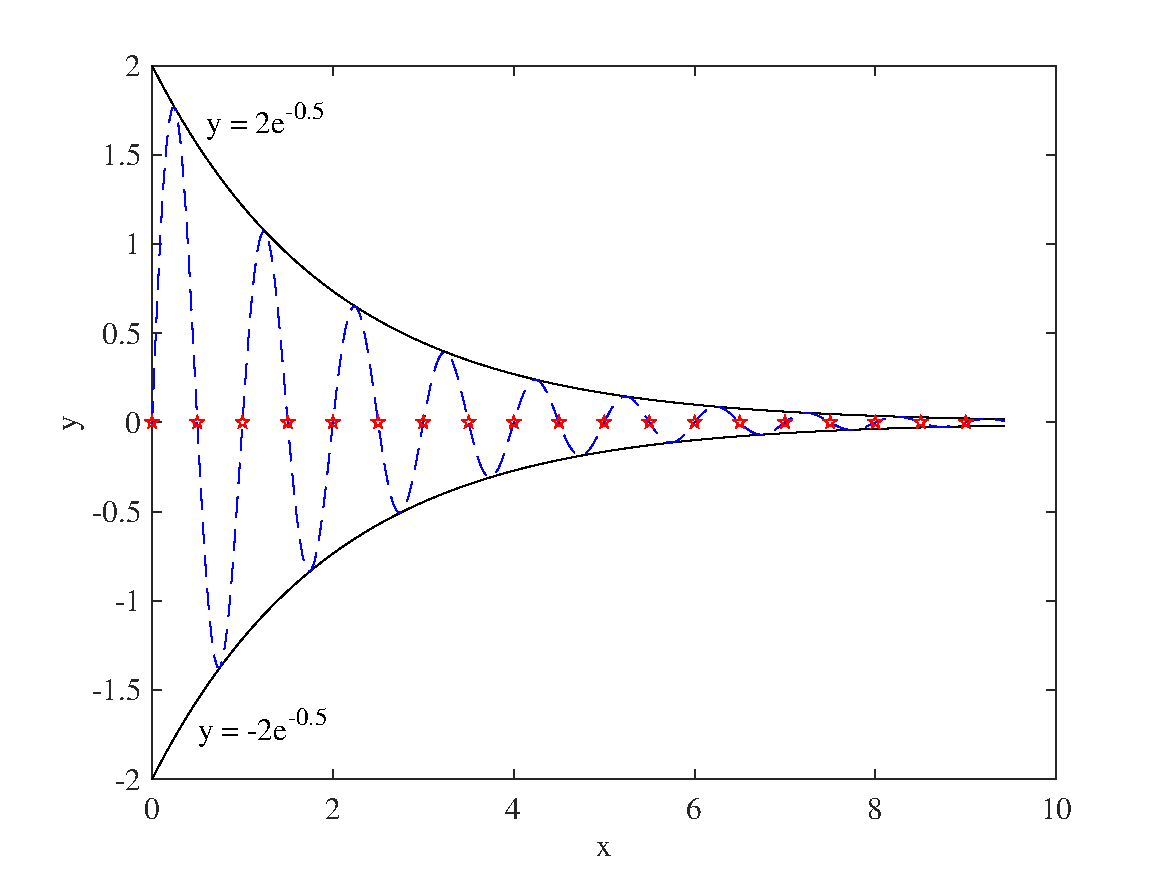
\includegraphics[width=0.7\linewidth]{pic/绘图1.pdf}
	\vspace*{-1.5em}
	\caption{\ref{EX41}输出结果图}
\end{figure}

\subsection{图形的辅助操作}
常见的辅助操作如下表
\begin{table}[!htb]
	\centering
	\setlength{\tabcolsep}{5mm}{
		\begin{tabular}{cll}
			\toprule
			功能 & 函数 & 说明 \\
			\midrule
			\multirow{5}*{ 图形标注 } & \lstinline|title(图形名称)| & 图形的标题\\
			& \lstinline|xlabel(x轴说明)| & $x$ 轴的标签\\
			& \lstinline|ylabel(y轴说明)| & $y$ 轴的标签\\
			& \lstinline|zlabel(z轴说明)| & $z$ 轴的标签\\
			& \lstinline|legend(图例1, 图例2, ……)| & 曲线的图例\\
			\hline
			\multirow{7}*{ 坐标轴控制 } & \lstinline|axis([xmin, xmax, ymin, ymax, zmin, zmax])|& 有几个特殊用法\\
			& \lstinline|axis equal| & 坐标采用等长刻度  \\ 
			& \lstinline|axis square| & 产生正方形坐标系  \\ 
			& \lstinline|axis auto|  & 默认设置  \\ 
			& \lstinline|axis on/off| & 显示/取消坐标轴 \\ 
			& \lstinline|grid on/off| & 打开/关闭网格线\\
			& \lstinline|box on/off| & 加/不加边框线\\
			\hline
			图像窗口的控制 & \lstinline|subplot(m, n, p)| & \makecell[l]{划分$m\times n$个绘图区,\\选定第$p$个区块绘制}\\
			\bottomrule
		\end{tabular}
	}
\end{table}
\vspace*{-0.5em}

\examples\label{EX42}
\begin{lstlisting}
x = 0 : 2*pi/60 : 2*pi;
y = sin(x);	z = cos(x);
t = sin(x) ./ (cos(x) + eps);	ct = cos(x) ./ (sin(x) + eps);
subplot(2, 2, 1);
plot(x, y-1);
title('sin(x) - 1');	axis([0, 2*pi, -2, 0]);
subplot(2, 1, 2);
plot(x, z-1);
title('cos(x) - 1');	axis([0, 2*pi, -2, 0]);
subplot(4, 4, 3);
plot(x, y);
title('sin(x)');	axis([0, 2*pi, -1, 1]);
subplot(4, 4, 4);
plot(x, z);
title('cos(x)');	axis([0, 2*pi, -1, 1]);
subplot(4, 4, 7);
plot(x, t);
title('tan(x)');	axis([0, 2*pi, -40, 40]);
subplot(4, 4, 8);
plot(x, ct);
title('cot(x)');	axis([0, 2*pi, -40, 40]);
\end{lstlisting}

输出结果如图\ref{OEX42}.
\begin{figure}[!htb]
	\centering
	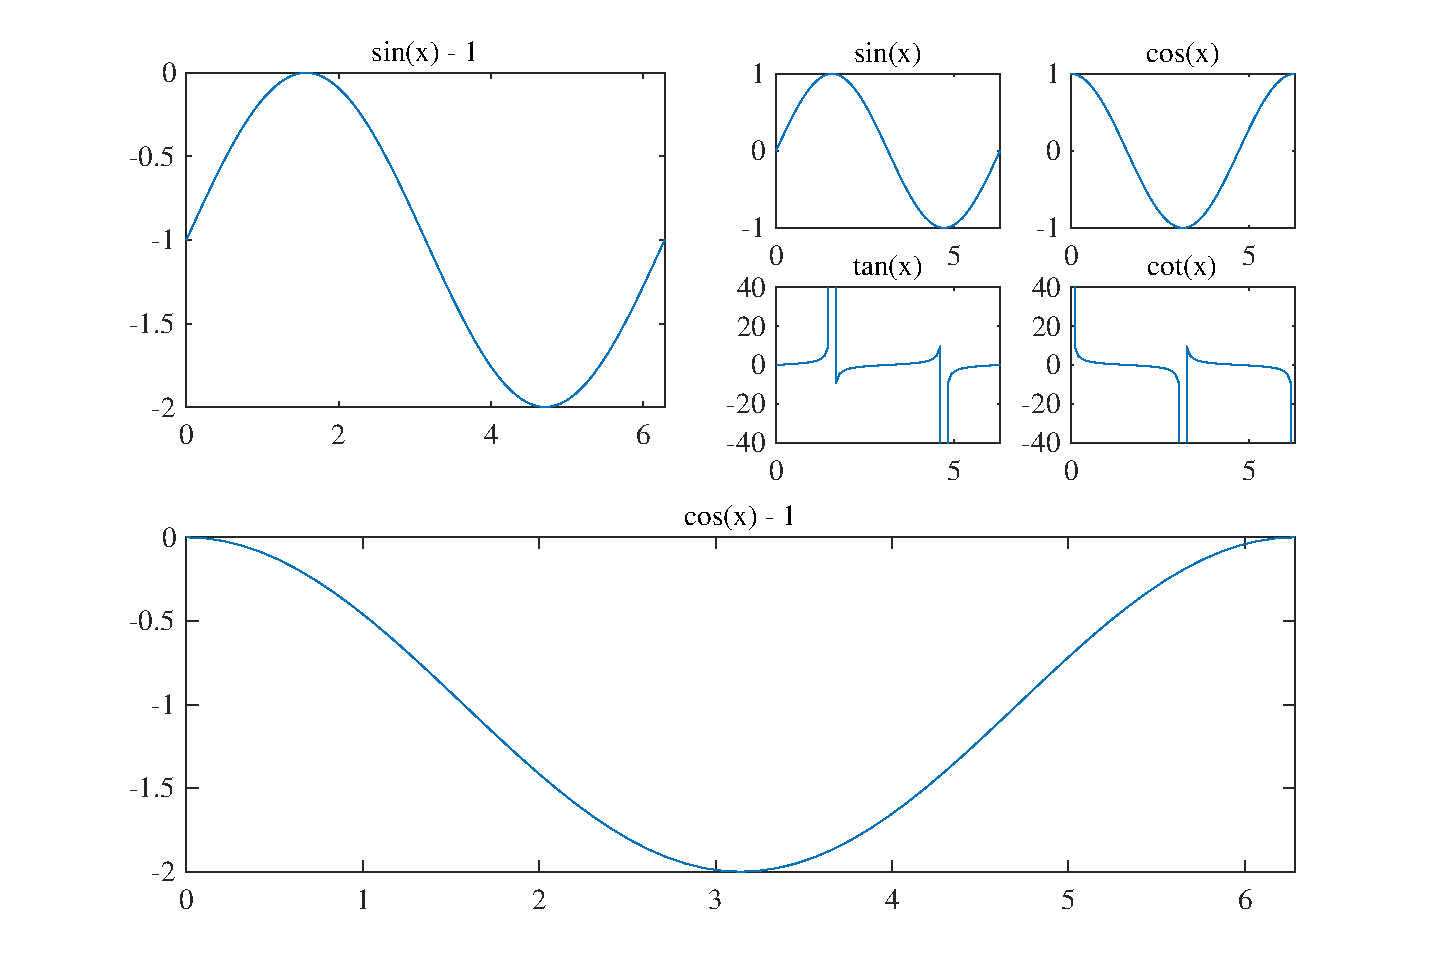
\includegraphics[width=0.8\linewidth]{pic/绘图2.pdf}
	\vspace*{-1.5em}
	\caption{\ref{EX42}输出结果图}
	\label{OEX42}
\end{figure}

\section{其他形式的二维图形}
\subsection{其他坐标系下的二维曲线图}
\begin{table}[!htb]
	\centering
	\setlength{\tabcolsep}{3mm}{
		\begin{tabular}{cll}
			\toprule
			功能 & 函数 & 说明 \\
			\midrule
			\multirow{3}*{ 对数坐标系 } & \lstinline|semilogx(x1,y1,选项1, x2,y2,选项2, ...)| & $x$轴对数刻度,$y$轴线性刻度\\
			& \lstinline|semilogy(x1,y1,选项1, x2,y2,选项2, ...)| & $x$ 轴线性刻度,$y$轴对数刻度\\
			& \lstinline|loglog(x1,y1,选项1, x2,y2,选项2, ...)| & $x$ 轴对数刻度,$y$轴对数刻度\\
			\hline
			极坐标系 & \lstinline|polar(theta, rho, 选项)| & theta为极坐标极角,rho为极坐标极径\\
			\bottomrule
		\end{tabular}
	}
\end{table}

注:选项与\lstinline|plot|的选项用法一致。

\examples \label{EX43}绘制蝴蝶曲线$\displaystyle \rho = \e^{\cos \theta}- 2\cos(4\theta)+\sin^5\dfrac{\theta}{12}$.
\vspace*{1em}
\begin{lstlisting}
t = 0:pi/50: 20*pi;
r1 = exp(cos(t)) - 2*cos(4*t) + sin(t/12).^5;
r2 = exp(cos(t - pi/2)) - 2*cos(4*(t - pi/2)) + sin((t - pi/2)/12).^5;
subplot(1, 2, 1)
polar(t, r1)
subplot(1, 2, 2)
polar(t, r2)
\end{lstlisting}

输出结果如图\ref{OEX43}.
\begin{figure}[!htb]
	\centering
	\vspace*{-1em}
	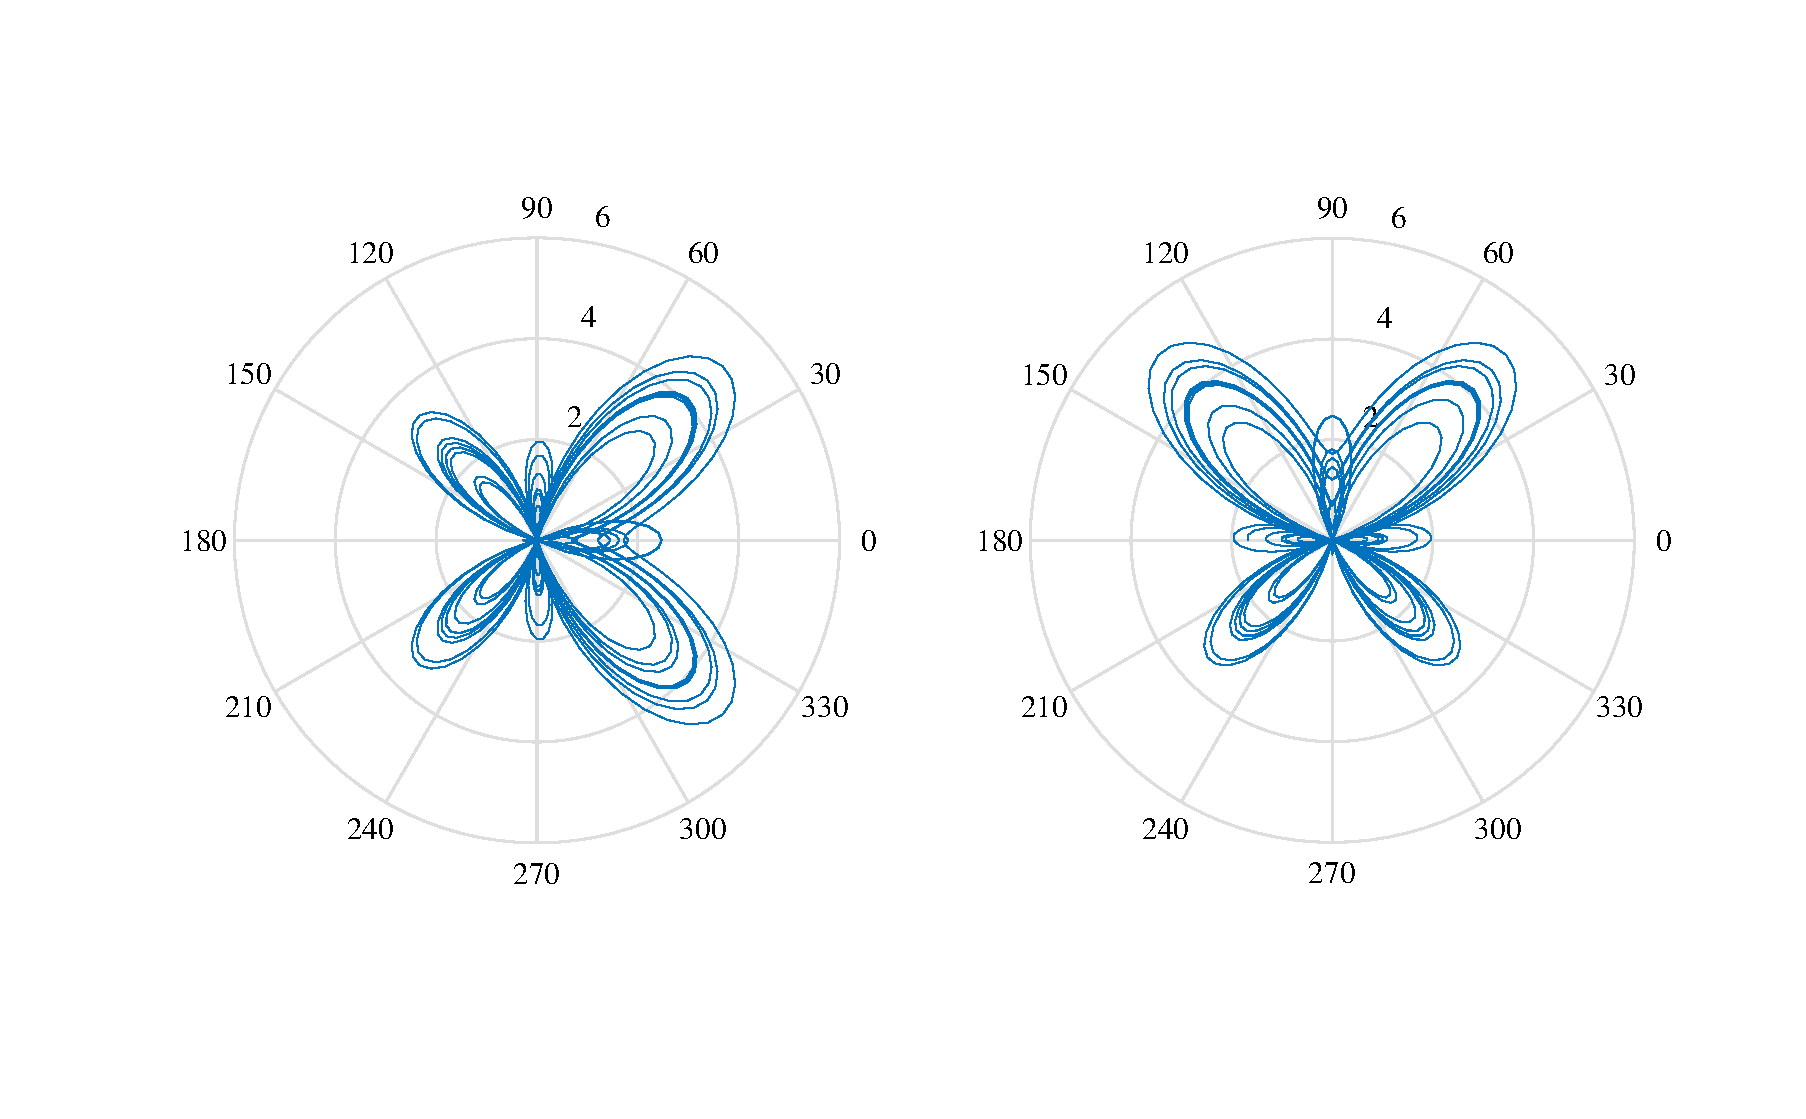
\includegraphics[width=0.8\linewidth]{pic/极坐标图.pdf}
	\vspace*{-5em}
	\caption{\ref{EX43}输出结果图}
	\label{OEX43}
\end{figure}
\subsection{条形类图形}
\label{条形类}
\begin{enumerate}
	\item 条形图\\
	绘制二维条形图的函数为\lstinline|bar|(垂直条形图)和\lstinline|barh|(水平条形图),它们的调用格式是一致的。以\lstinline|bar|为例
	\begin{itemize}
		\item \lstinline|bar(y)|
		\begin{itemize}
			\item 若$y$为向量,则分别显示每个分量的高度,横坐标为$y$的下标
			\item 若$y$为矩阵,则分别比较每一行的大小,横坐标为矩阵的行数
		\end{itemize}
		\item \lstinline|bar(x, y, style)|
		\begin{itemize}
			\item 当$y$是$m \times n$的矩阵时,矩阵中每一行元素绘制在一组中,每组的横坐标为对应$x$的行元素
			\item \lstinline|style|指定条形的排列模式,可选的有\lstinline|grouped|(簇状分组)和\lstinline|stacked|(堆积分组),默认采用\lstinline|grouped|
		\end{itemize}
	\item 例子
	\begin{lstlisting}
x = -1:1;
y = [1,2,3,4,5; 1,2,1,2,1; 5,4,3,2,1];
subplot(1,2,1);	bar(x,y,'grouped');
title('Group');	axis([-3,3, 0,6]);
subplot(1,2,2);	barh(x,y,'stacked')
title('Stack');
	\end{lstlisting}
\begin{figure}[!htb]
	\centering
	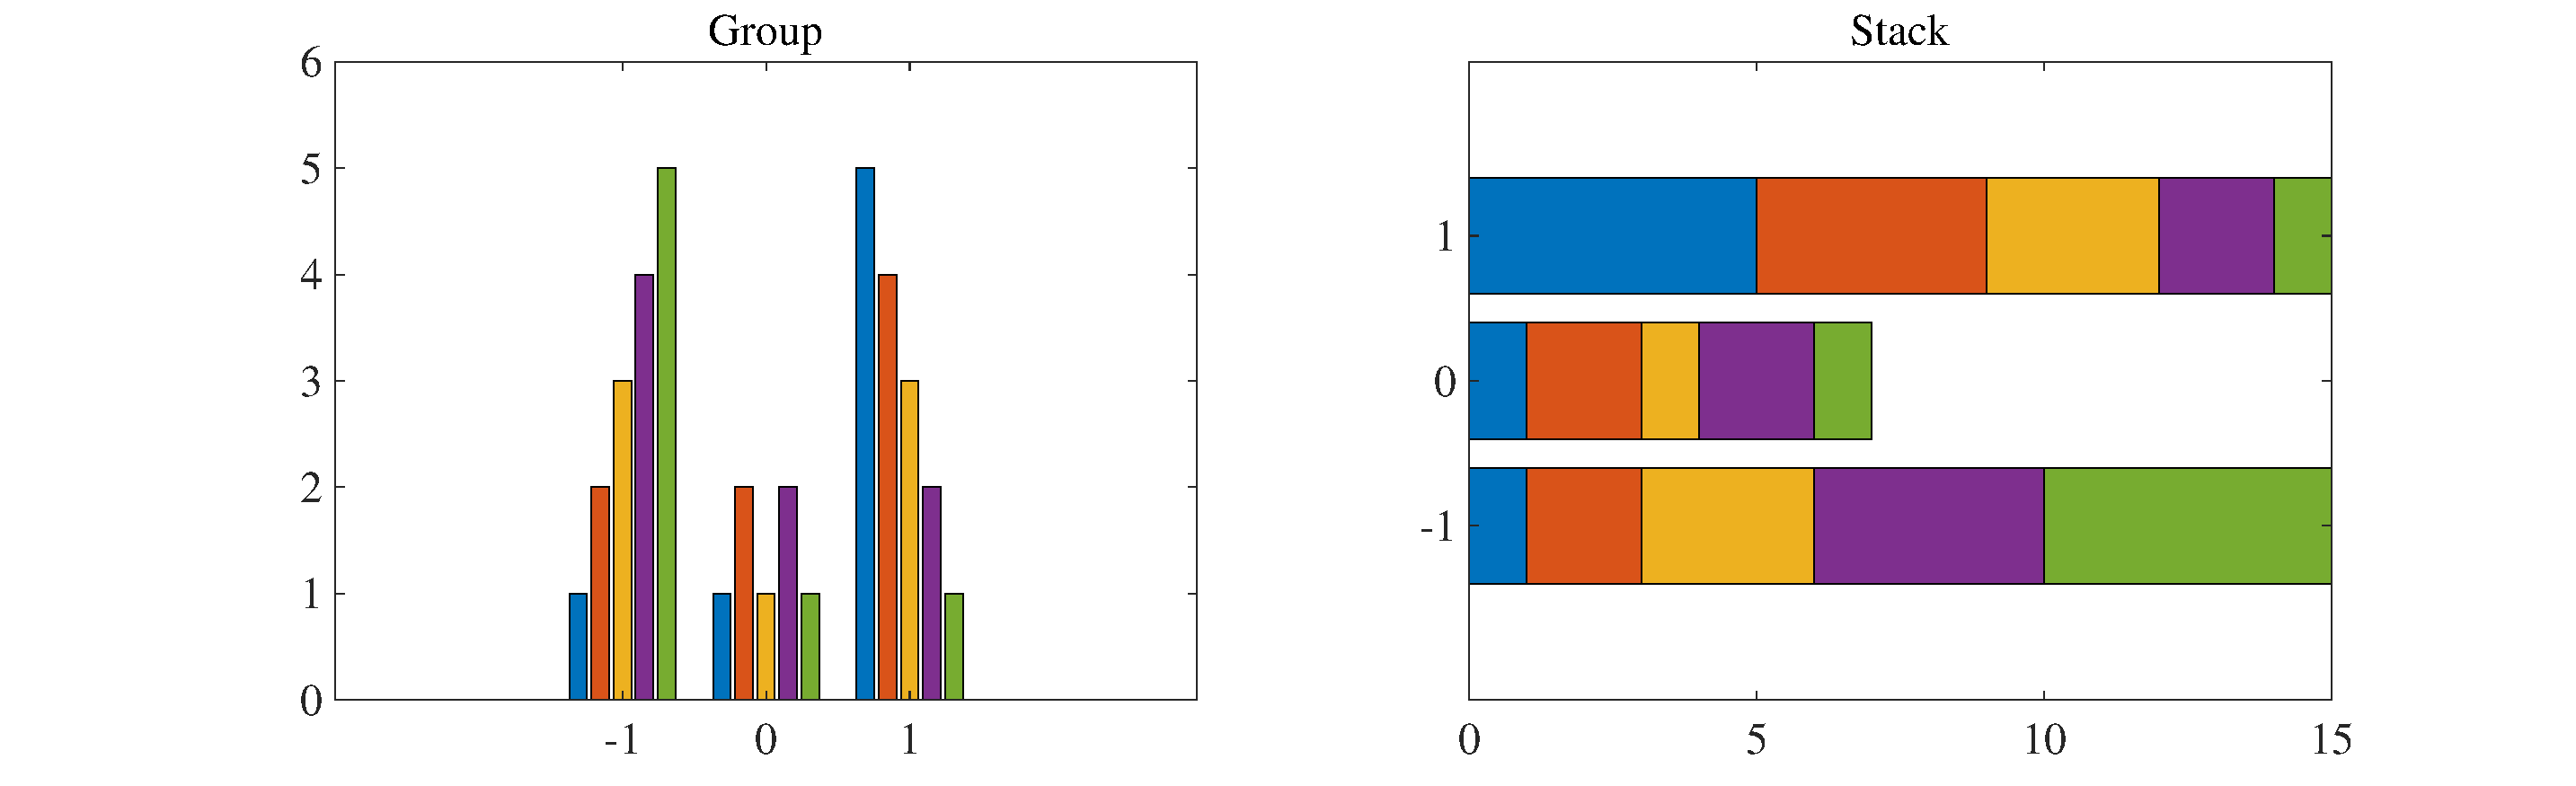
\includegraphics[width=\linewidth]{pic/条形图.pdf}
	\caption{条形图}
\end{figure}
	\end{itemize}
\item 直方图
\begin{itemize}
	\item \lstinline|hist(y, x)|
	\begin{itemize}
		\item 若$y$为向量,则将其最小值与最大值的区间等分,并统计每个区间元素的个数,然后以元素个数为高度绘制条形图
		\item 若$y$为矩阵,将$y$的每一列作为一个向量,绘制每一列元素的直方图
		\item 若$x$为标量,则统计区间均分成$x$个小区间
		\item 若$x$为向量,则区间数为向量的长度,向量中的每一个数为各个区间的中心点
	\end{itemize}
	\item \lstinline|rose(theta, x)|
		\begin{itemize}
		\item 向量\lstinline|theta|用于确定每一区间的长度,每一区间的长度反映出在该区间的\lstinline|theta|元素个数
		\item 若$x$为标量,则在$[0, 2\pi]$区间内画出$x$个等角度的小扇形,默认值为20
		\item 若$x$为向量,则$x$指定分组中心值,$x$元素个数为数据分组数。
	\end{itemize}
		\item 例子
	\begin{lstlisting}
y = randn(500,1);
subplot(2,2,1);	
hist(y);	title('高斯分布直方图')
x = -4:0.1:4;
subplot(2,2,2);	
hist(y, x);	title('指定范围的高斯分布直方图')
subplot(2,1,2);	
theta = y * pi;
rose(theta);	title('在极坐标下的直方图')
	\end{lstlisting}
	\begin{figure}[!htb]
		\centering
		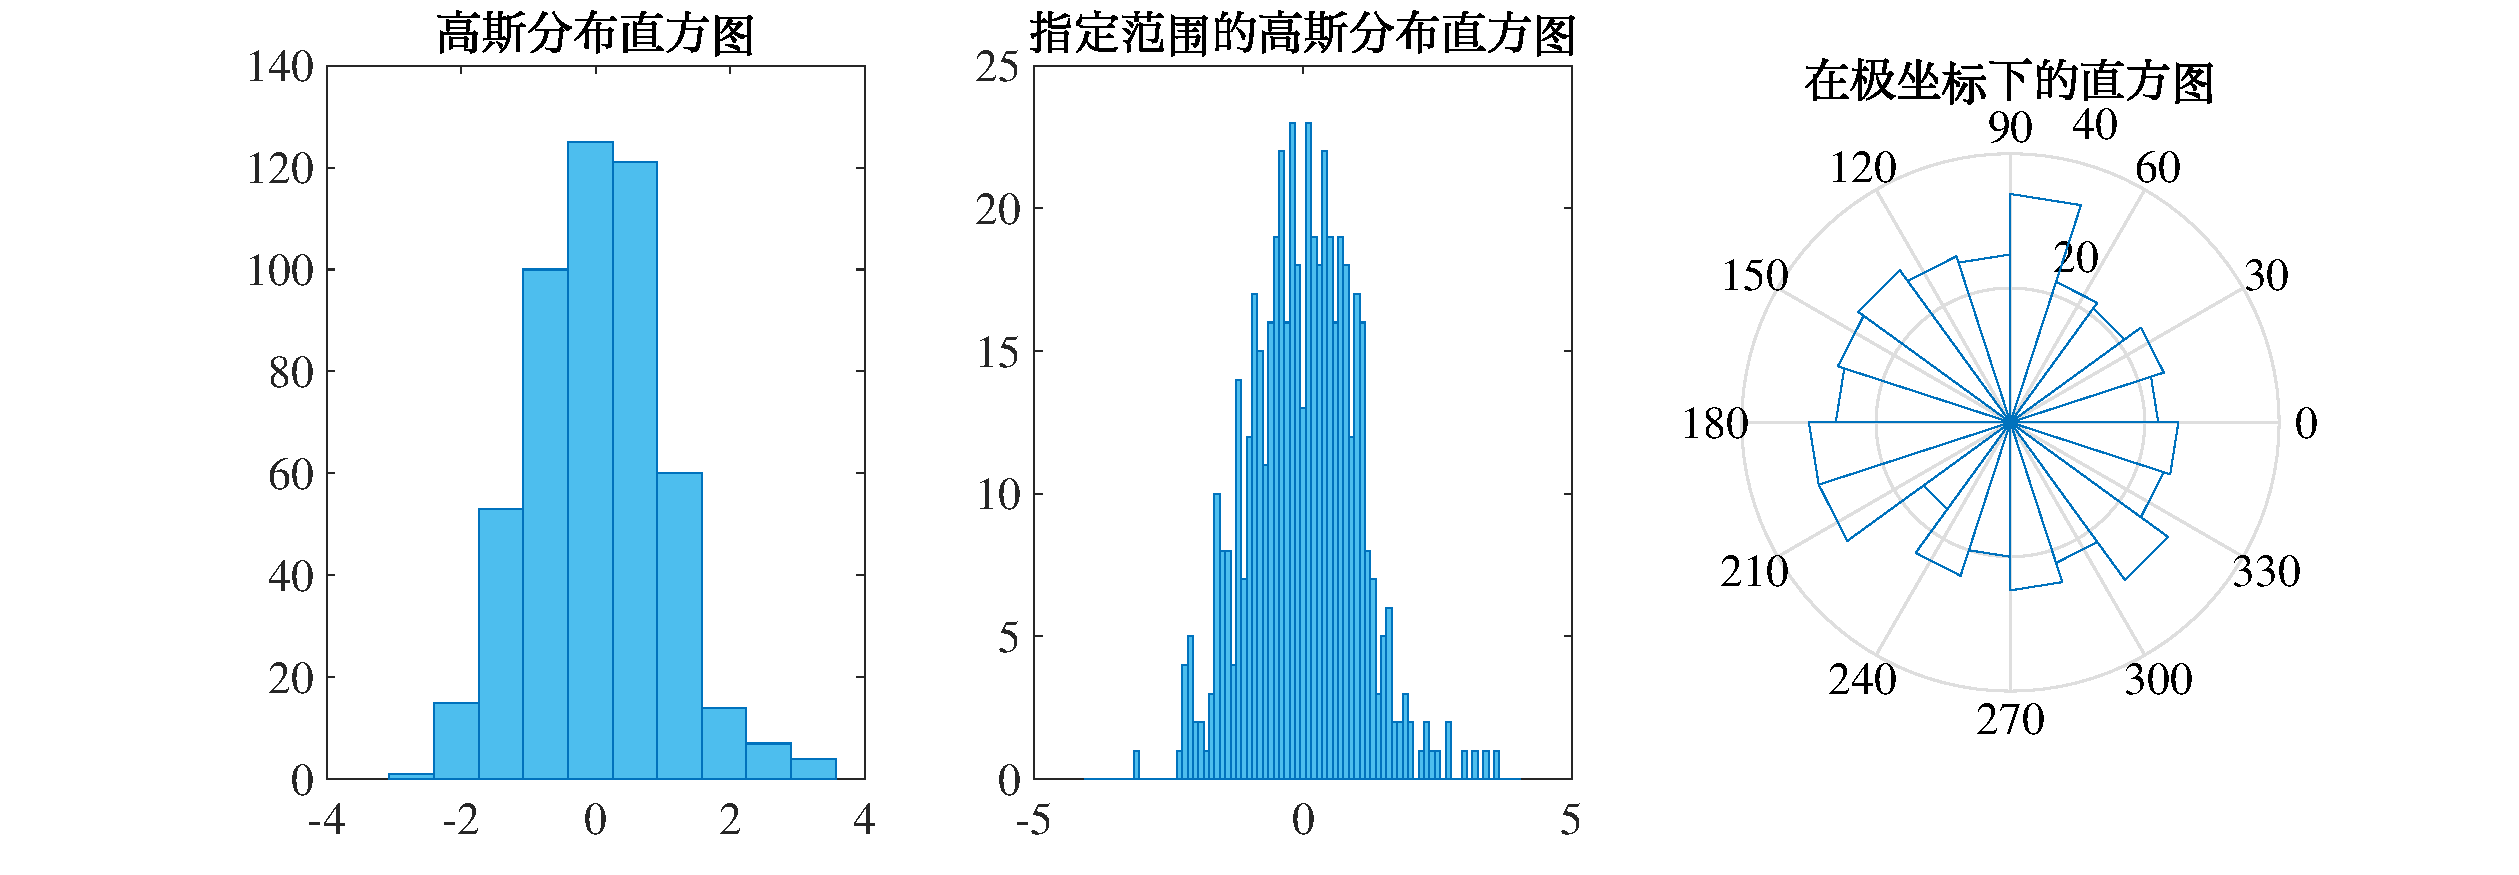
\includegraphics[width=\linewidth]{pic/直方图.pdf}
		\caption{直方图}
	\end{figure}
\end{itemize}
\end{enumerate}

\newpage 

\subsection{面积类图形}
\begin{enumerate}
	\item 扇形统计图
	\begin{itemize}
		\item \lstinline|pie(x, explode)|
		\begin{itemize}
			\item $x$为向量,$x$的每个元素占有一个扇形,从饼图的正上方开始,按逆时针顺序绘制。
			\item $x$为矩阵,则将矩阵的所有元素按序号一个个绘制扇形
			\item 若$x$的元素之和小于1,则绘制的图形不是一个完整的圆
			\item \lstinline|explode|是与$x$同等大小的向量或矩阵,与\lstinline|explode|的非零值对应的部分将从饼图中心分离出来
		\end{itemize}
	\item 例子
	\begin{lstlisting}
pie([7,17,23,19,5], [0,0,0,0,1]);
title('pie map');
legend('A', 'A-', 'B', 'C', 'D');
	\end{lstlisting}
\begin{figure}[!htb]
	\centering
	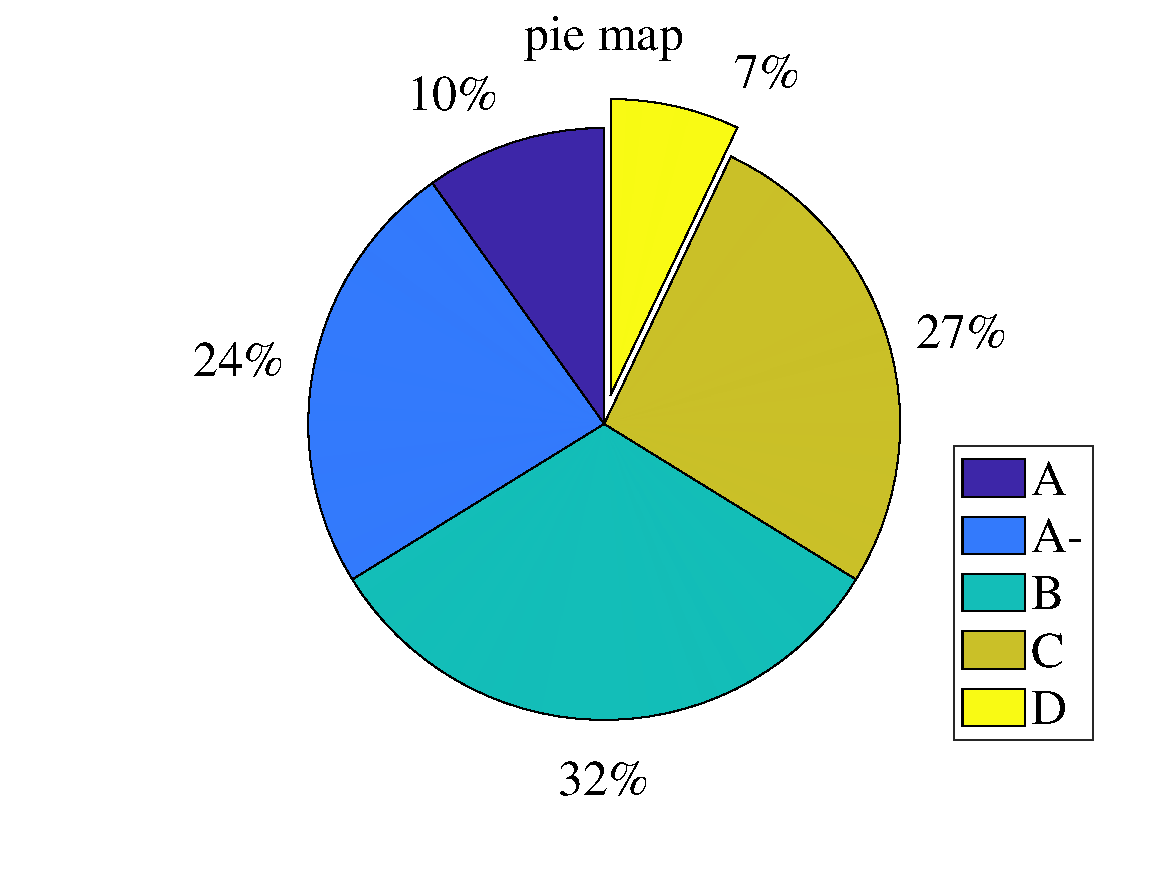
\includegraphics[width=0.5\linewidth]{pic/饼图.pdf}
	\caption{饼图}
\end{figure}
	\end{itemize}
	\item 面积统计图
	\begin{itemize}
		\item \lstinline|area(x, y)|
		\begin{itemize}
			\item $x,y$都是向量,与\lstinline|plot(x, y)|一样,但将所得曲线下方填色
			\item $x$为向量,$y$为矩阵,则矩阵但每一列与向量$x$成对绘图
		\end{itemize}
		\item 例子
	\begin{lstlisting}
x = 1:2:9;
y = [1,3,5,2,6; 2,4,5,6,2; 5,4,7,2,2]
area(x, y);	
grid on; 
title('Area map');
	\end{lstlisting}
	\begin{figure}[!htb]
		\centering
		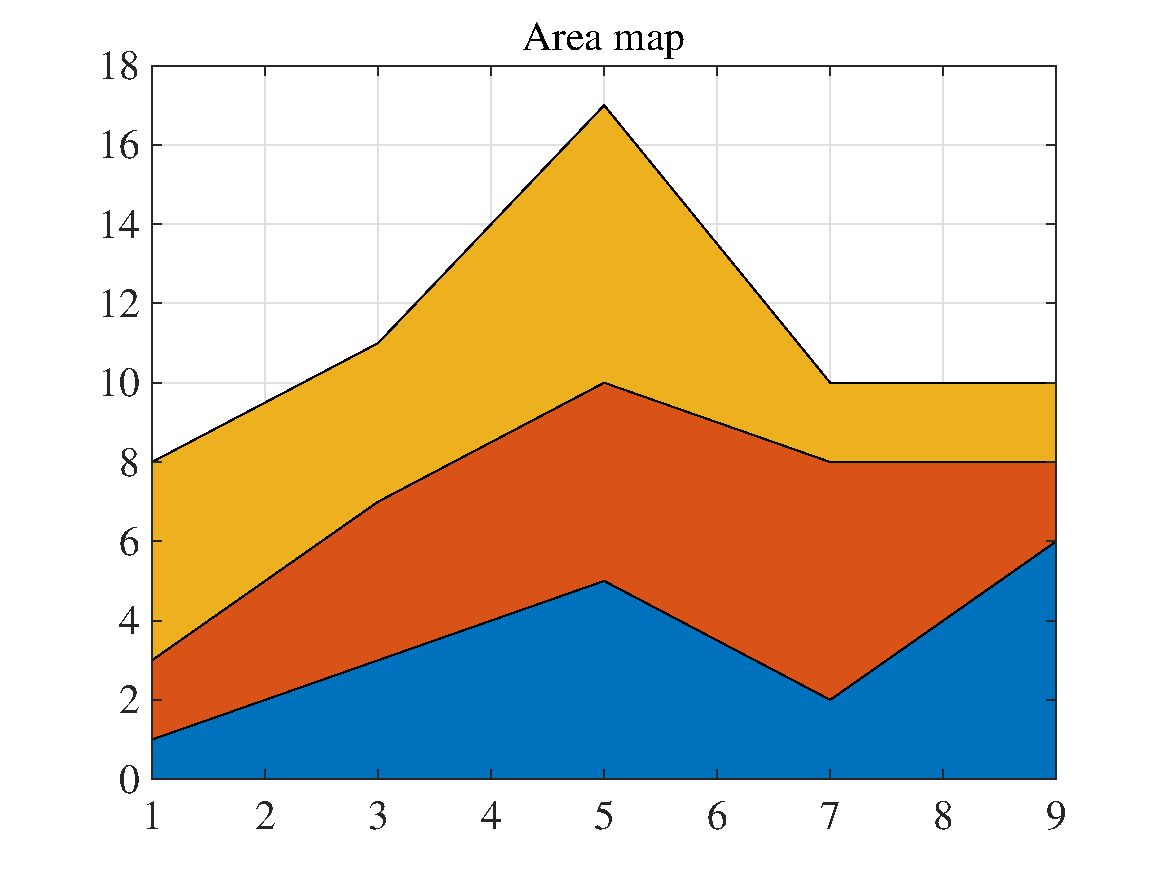
\includegraphics[width=0.6\linewidth]{pic/面积图.pdf}
		\caption{面积图}
	\end{figure}
	\end{itemize}
\item 实心图
\begin{itemize}
	\item \lstinline|fill(x, y, color)|
	\begin{itemize}
		\item 按向量$x,y$下标增加的方向依次连接点$(x_i,y_i)$,若最后首尾不封闭,那么将自动首尾相连,构成封闭多边形,然后内部涂色。
	\end{itemize}
		\item 例子
\begin{lstlisting}
t = 0: 2*pi/1000:2*pi;
x = sin(t);
y = cos(t);
fill(x,y,'k');
axis equal; axis([-1.5,1.5, -1.5,1.5]);
\end{lstlisting}
\begin{figure}[!htb]
	\centering
	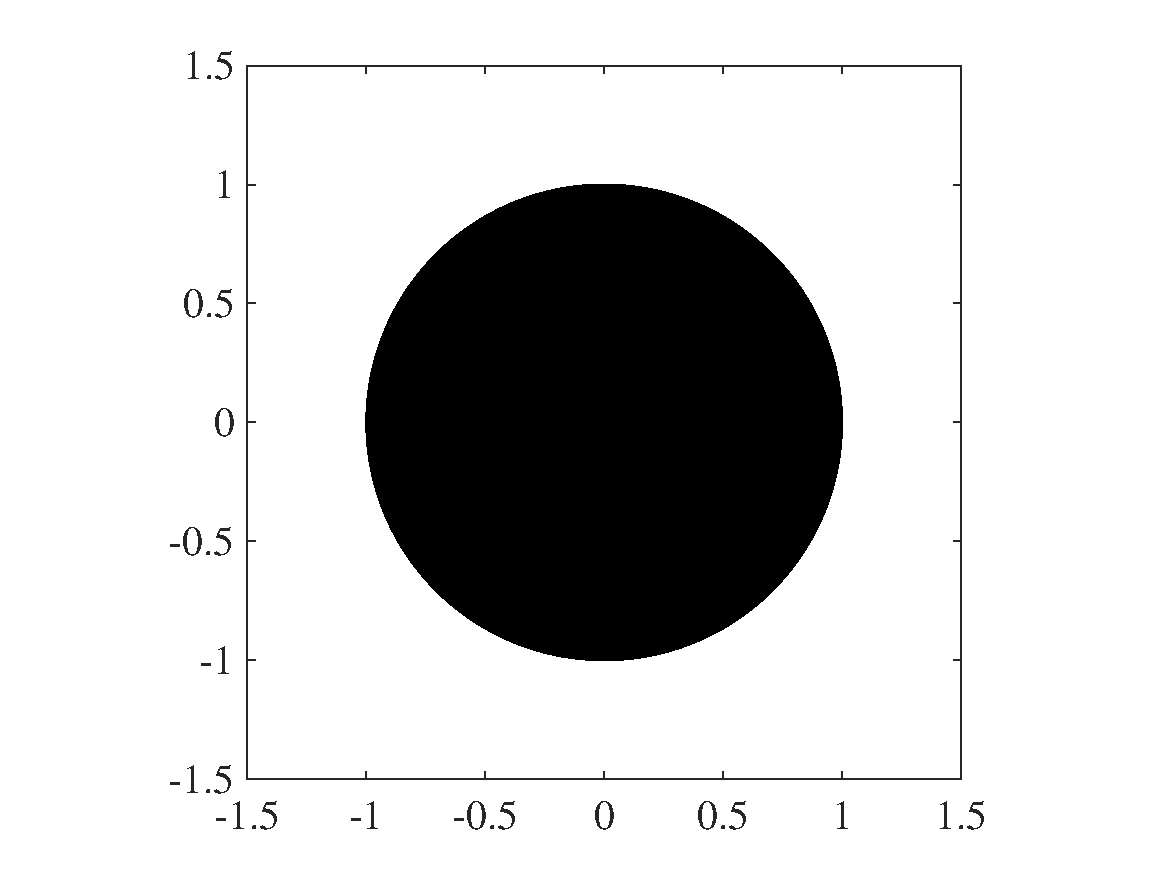
\includegraphics[width=0.6\linewidth]{pic/实心图.pdf}
	\caption{实心图}
\end{figure}
\end{itemize}
\end{enumerate}

\subsection{散点类图形}
\begin{itemize}
	\item 散点图:\lstinline|scatter(x, y, 'filled', color)|
	\item 阶梯图\lstinline|stairs(x, y, 选项)|
	\item 杆图:\lstinline|stem(x, y, 选项)|
\end{itemize}
其中,$x,y$为大小相同的向量,用于绘制点。例子
\begin{lstlisting}
x = 0:0.35:7;
y = 2*exp(-0.5*x);
subplot(1,3,1);	scatter(x, y, 'g');
title('scatter');	axis([0,7, 0,2]);
subplot(1,3,2); stairs(x,y,'b');
title('stairs');	axis([0,7, 0,2]);
subplot(1,3,3);	stem(x,y,'k');
title('stem');	axis([0,7, 0,2]);
\end{lstlisting}
\begin{figure}[!htb]
	\centering
	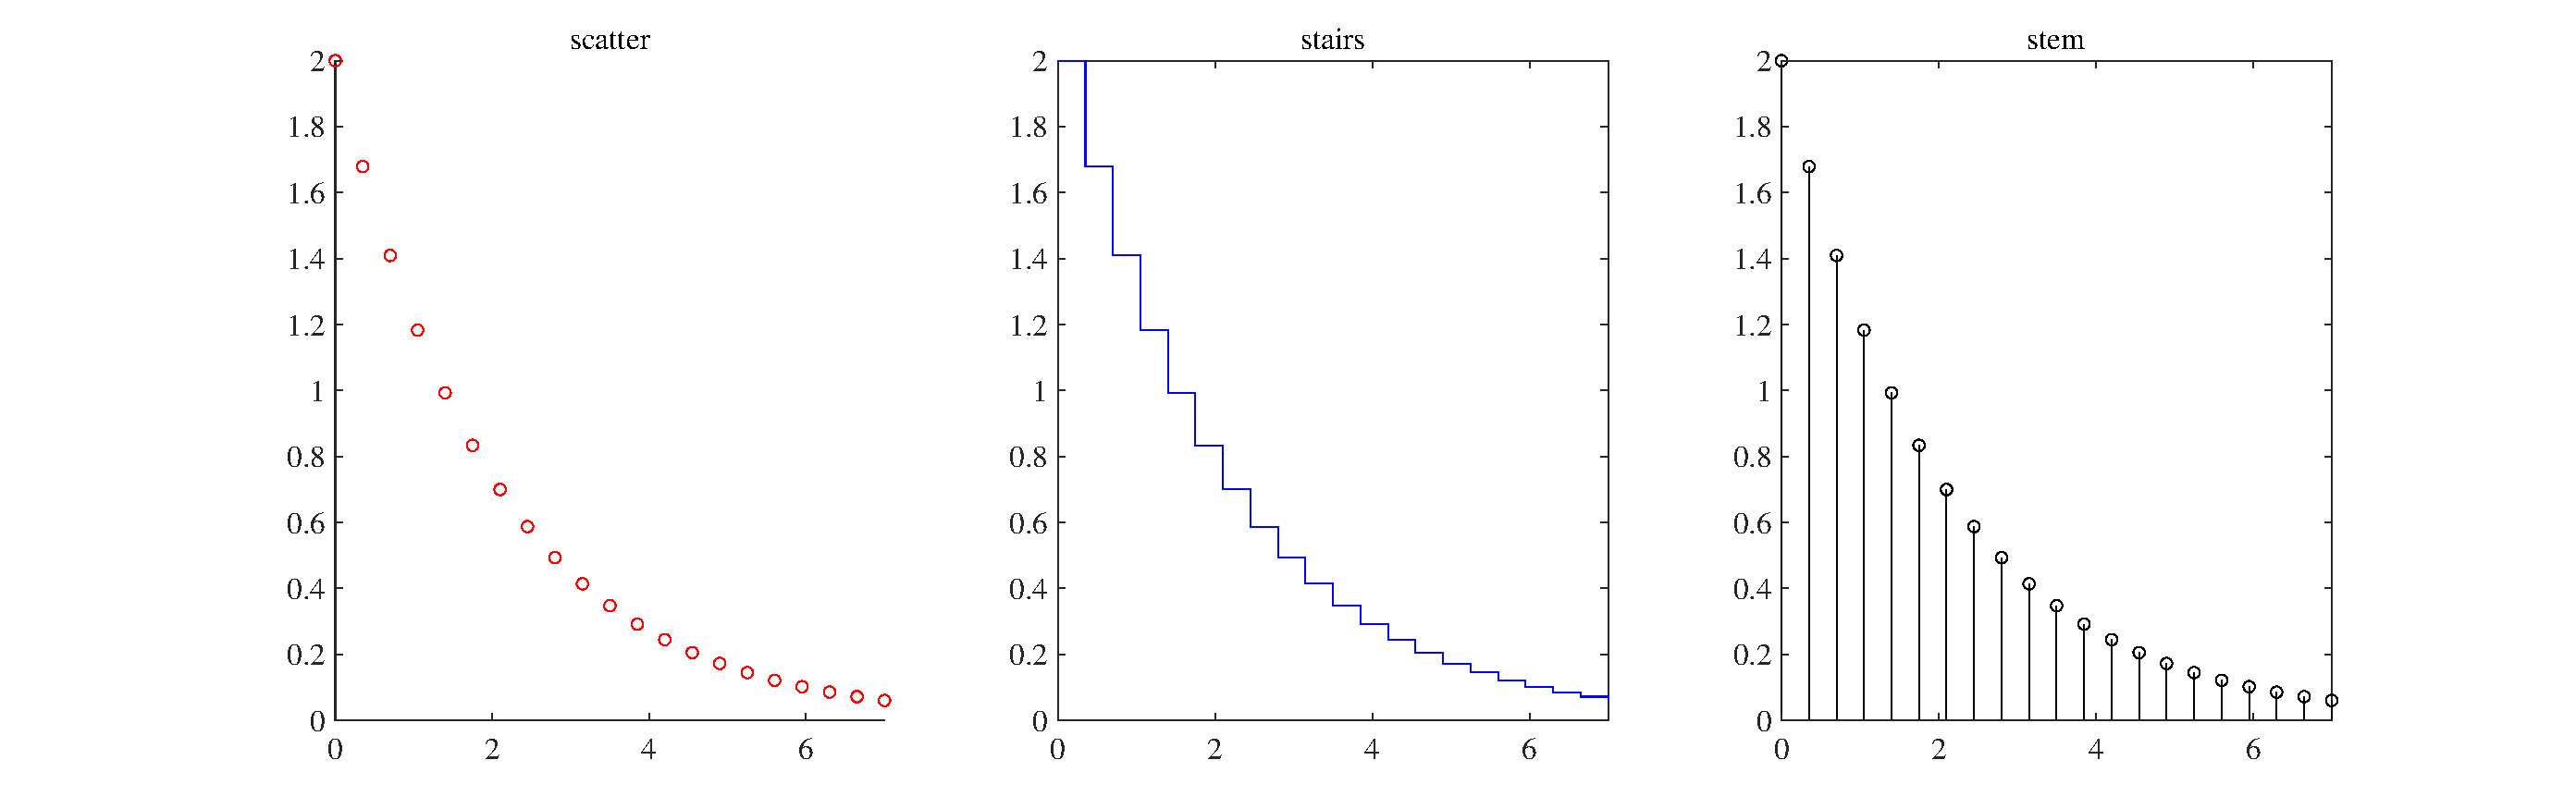
\includegraphics[width=\linewidth]{pic/散点图.pdf}
	\caption{散点图}
\end{figure}

\subsection{矢量类图形}
\label{矢量类}
\begin{enumerate}
	\item 罗盘图
	\begin{itemize}
		\item \lstinline|compass(x,y)|
		\begin{itemize}
			\item $x,y$为$n$个向量,显示$n$个箭头
			\item 箭头的起点为原点,终点为$(x_i,y_i)$.
		\end{itemize}
		\item \lstinline|compass(z)|
		\begin{itemize}
			\item $z$为$n$个复数向量,显示$n$个箭头
			\item 箭头的起点为原点,终点为$(\text{real}(z),\text{image}(z))$
		\end{itemize}
	\end{itemize}
	\item 羽毛图
	\begin{itemize}
		\item \lstinline|feather(x,y)|
		\begin{itemize}
			\item 绘制由$x,y$所确定的向量
		\end{itemize}
		\item \lstinline|feather(z)|
		\begin{itemize}
			\item 绘制由复数$z$所确定的向量,等价于\lstinline|feather(real(z), imag(z))|.
		\end{itemize}
	\end{itemize}
	\item 箭头图
	\begin{itemize}
		\item \lstinline|quiver(x, y, u, v)|
		\begin{itemize}
			\item $(x,y)$为矢量起点,若省略,则在平面上均匀选取若干个点作为起点
			\item $(u,v)$为矢量终点
		\end{itemize}
	\end{itemize}
\end{enumerate}
例子:
\begin{lstlisting}
x= -pi:pi/8:pi;
y = sin(x);
subplot(2, 2, 1); compass(x, y);
title('罗盘图');
subplot(2, 2, 2); feather(x, y)
title('羽毛图');
subplot(2, 1, 2); quiver(x, y);
title('箭头图');
\end{lstlisting}
\vspace*{-1.5em}
\begin{figure}[!htb]
	\centering
	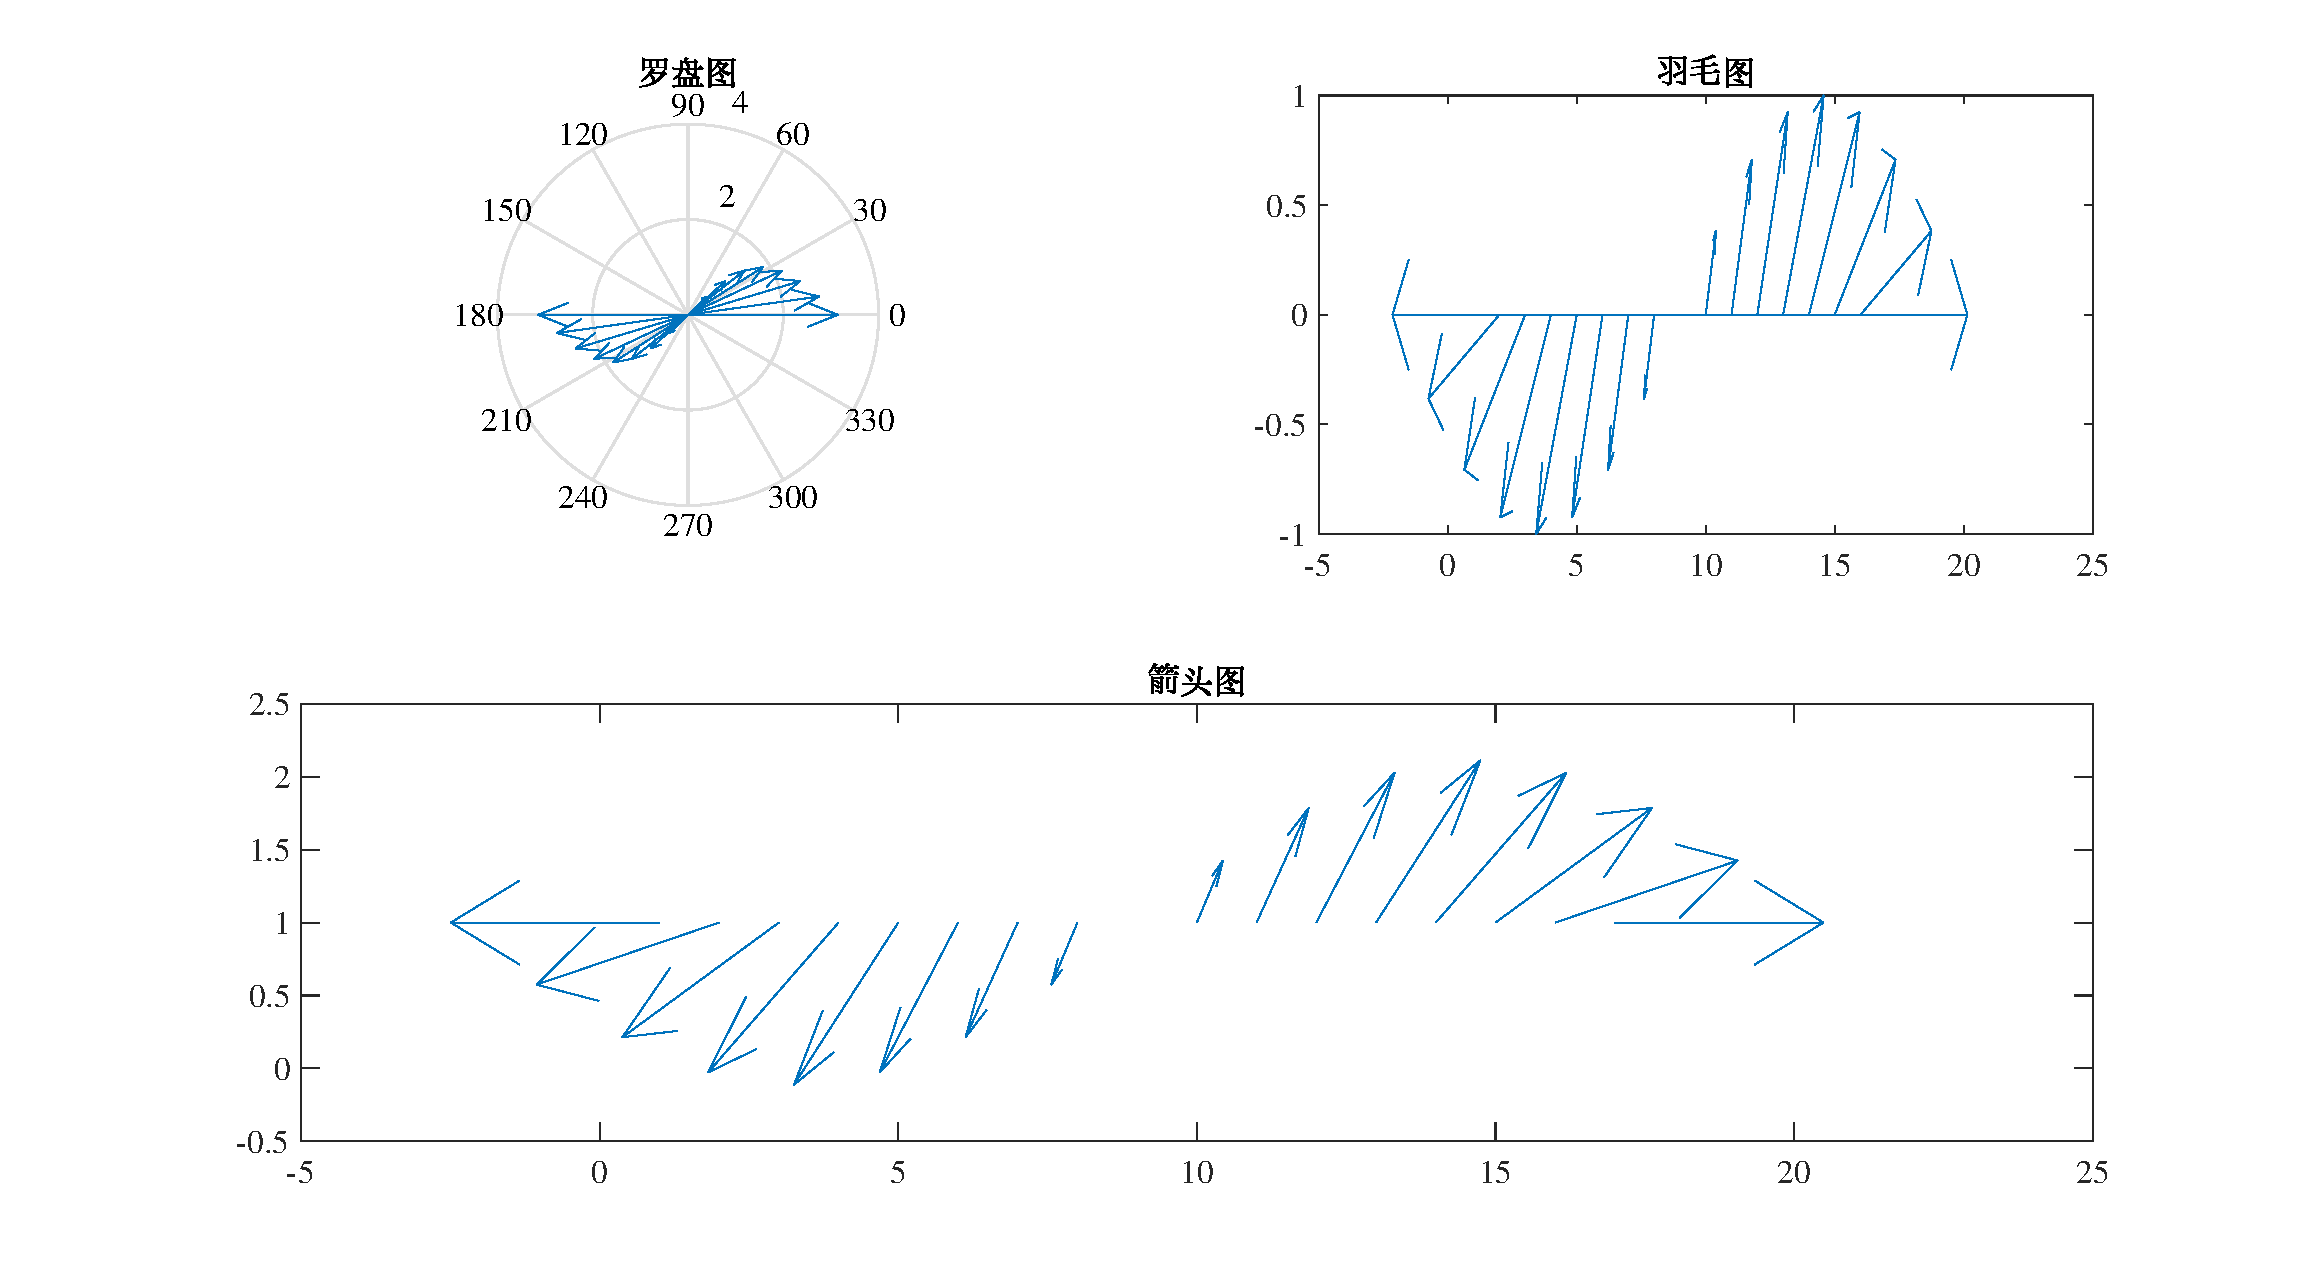
\includegraphics[width=\linewidth]{pic/二维矢量图.pdf}
	\vspace*{-3em}
	\caption{3种二维矢量类图形}
\end{figure}

\section{三维图形}
\subsection{绘制三维曲线的基本函数}
绘制三维图形的函数为
\begin{center}
	\lstinline|plot3(x1,y1,z1,选项1, x2,y2,z2,选项2, ..., xn,yn,选项n)|
\end{center}
其调用格式与\lstinline|plot|函数基本一致。
\begin{itemize}
	\item 当$x,y,z$是同长度的向量时,则$x,y,z$构成一条三维曲线
	\item 当$x,y,z$是同型矩阵时,则以$x,y,z$对应的列向量绘制三维曲线,曲线条数等于矩阵列数
\end{itemize}

\examples 绘制空间曲线
\begin{align*}
	\begin{cases}
		x^2 + y^2 + z^2 = 64\\
		y + z = 0
	\end{cases}
	\quad \Longrightarrow \quad 
	\begin{cases}
		x = 8\cos t\\
		y = 4 \sqrt{2} \sin t\\
		z = - 4 \sqrt{2} \sin t
	\end{cases}
,\quad 0 \le t \le 2\pi
\end{align*}

\begin{lstlisting}
t = 0:pi/50:2*pi;
x = 8*cos(t);
y = 4*sqrt(2)*sin(t);
z = -4*sqrt(2)*sin(t);
plot3(x,y,z,'p');
title('Line in 3-D Space');
text(0,0,0,'origin');
xlabel('X'); ylabel('Y'); zlabel('Z'); grid;
\end{lstlisting}
\vspace*{-1.5em}
\begin{figure}[!htb]
	\centering
	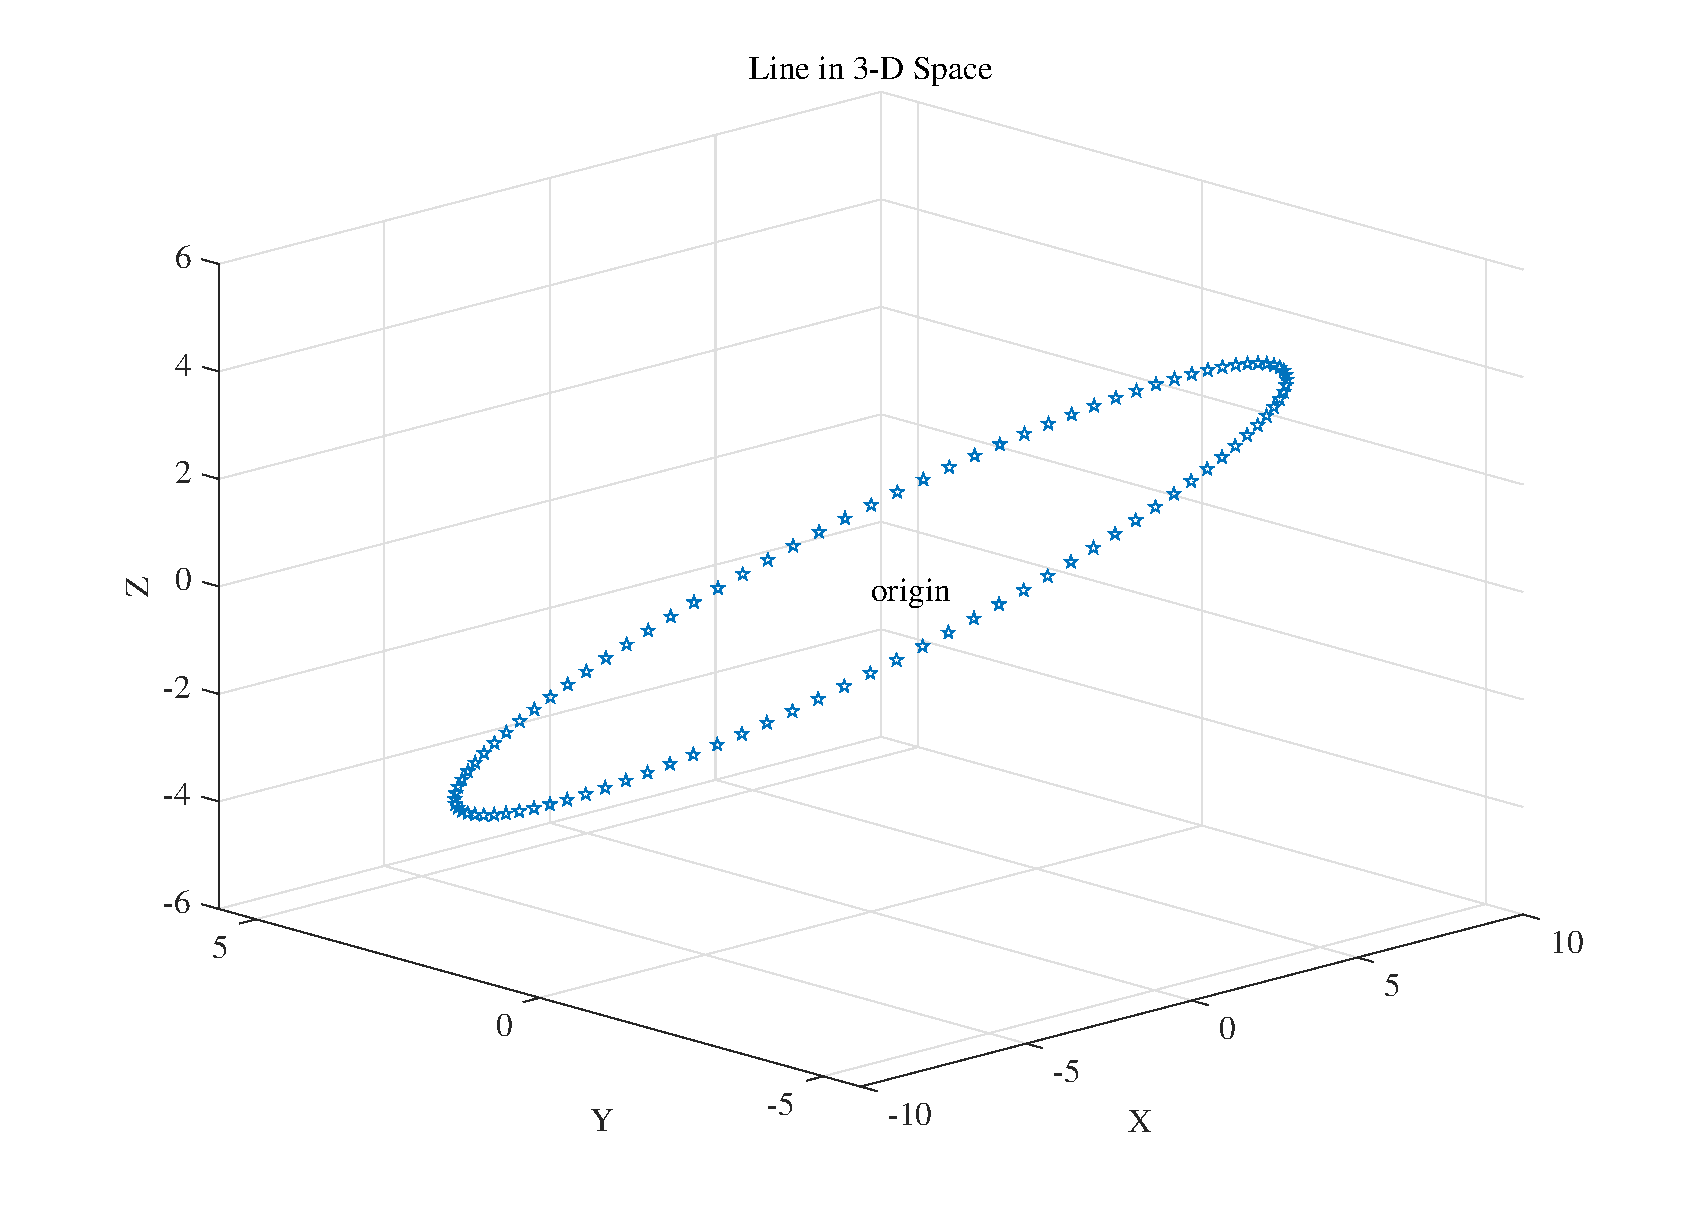
\includegraphics[width=0.8\linewidth]{pic/三维图1.pdf}
	\vspace*{-3em}
	\caption{三维曲线}
\end{figure}

\subsection{三维曲面}
\begin{enumerate}[1.]
	\item \textbf{平面网格坐标矩阵的生成}\\
	利用\lstinline|meshgrid|函数生成,调用格式如下
	\begin{lstlisting}
x = a:dx:b;
y = c:dy:d;
[X,Y] = meshgrid(x, y);
	\end{lstlisting}
当$\bm{x} = \bm{y}$时,可写作\lstinline|meshgrid(x)|.
	\item \textbf{绘制三维曲面的函数}
	\begin{itemize}
		\item \lstinline|mesh(x, y, c)|
		\item \lstinline|surf(x, y, c)|
	\end{itemize}
	一般情况下,$\bm{x},\bm{y},\bm{z}$是同型矩阵。
	\begin{itemize}
		\item $\bm{x}, \bm{y}$是网格坐标矩阵
		\item $\bm{z}$是网格点上的高度矩阵
		\item c称为色标矩阵,用于指定曲面的颜色。当c省略时,默认c = z,即颜色的设定与高度成正比,这样就可以得到层次分明的三维图形
		\item 当$\bm{x},\bm{y}$省略时,矩阵以$\bm{z}$的行下标为$x$坐标,列下标为$y$坐标绘制图形
	\end{itemize}
\end{enumerate}
\begin{lstlisting}
x = 0:0.1:2*pi;
[x, y] = meshgrid(x);
z = sin(y).*cos(x);
mesh(x,y,z);
xlabel('x'),ylabel('y'),zlabel('z');
title('mesh');
surf(x,y,z);
xlabel('x'),ylabel('y'),zlabel('z');
title('surf');
plot3(x,y,z);
xlabel('x'),ylabel('y'),zlabel('z');
title('plot3');
\end{lstlisting}
\begin{figure}[!htb]
	\centering
	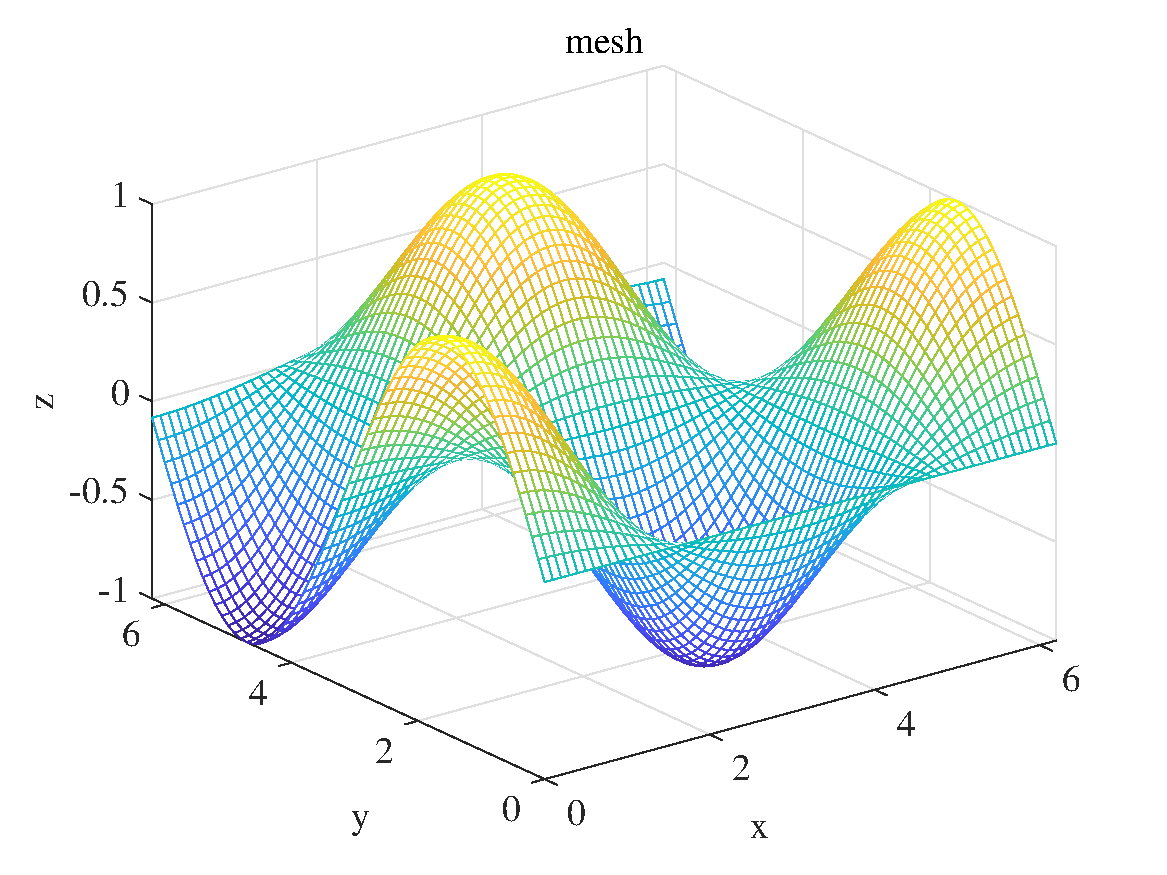
\includegraphics[width=0.7\linewidth]{pic/mesh.pdf}
	\vspace*{-2em}
	\caption{三维网格图}
\end{figure}
\begin{figure}[!htb]
	\centering
	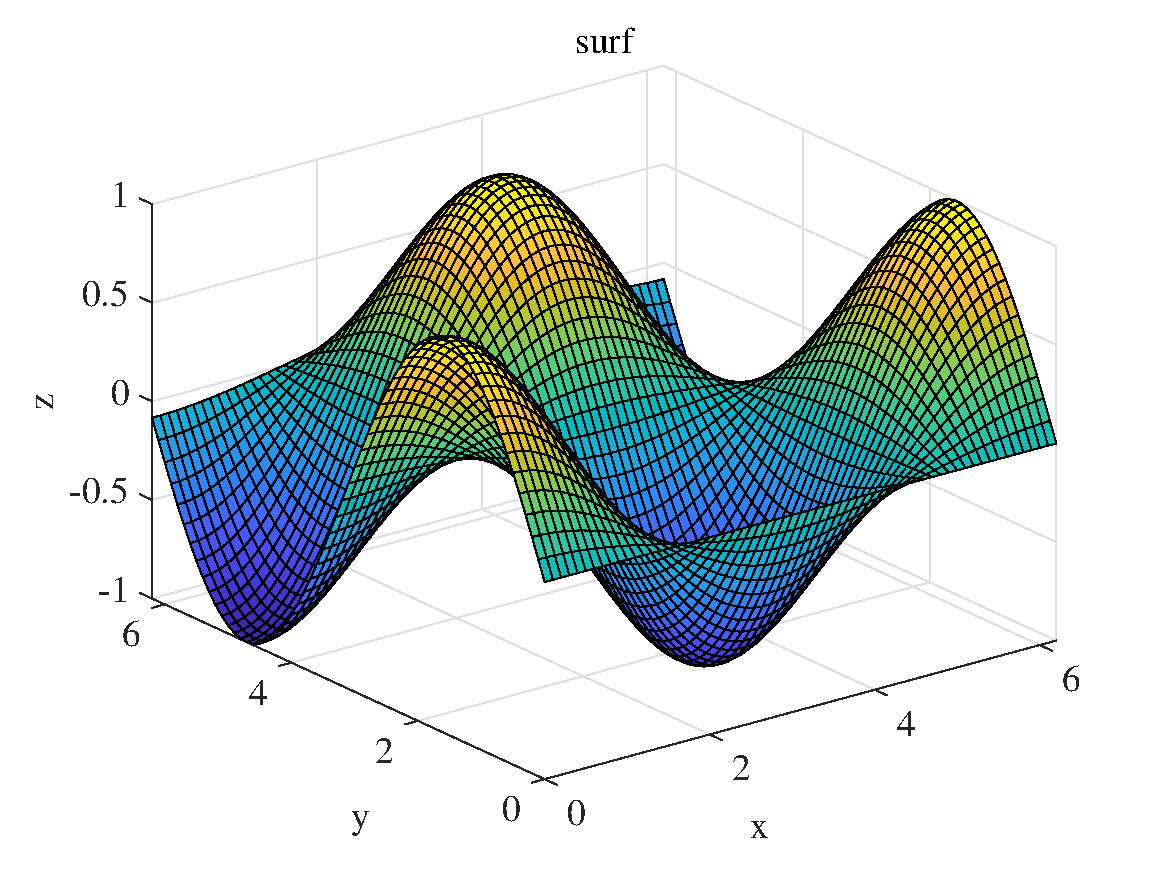
\includegraphics[width=0.6\linewidth]{pic/surf.pdf}
	\vspace*{-2em}
	\caption{三维曲面图}
\end{figure}
\begin{figure}[!htb]
	\centering
	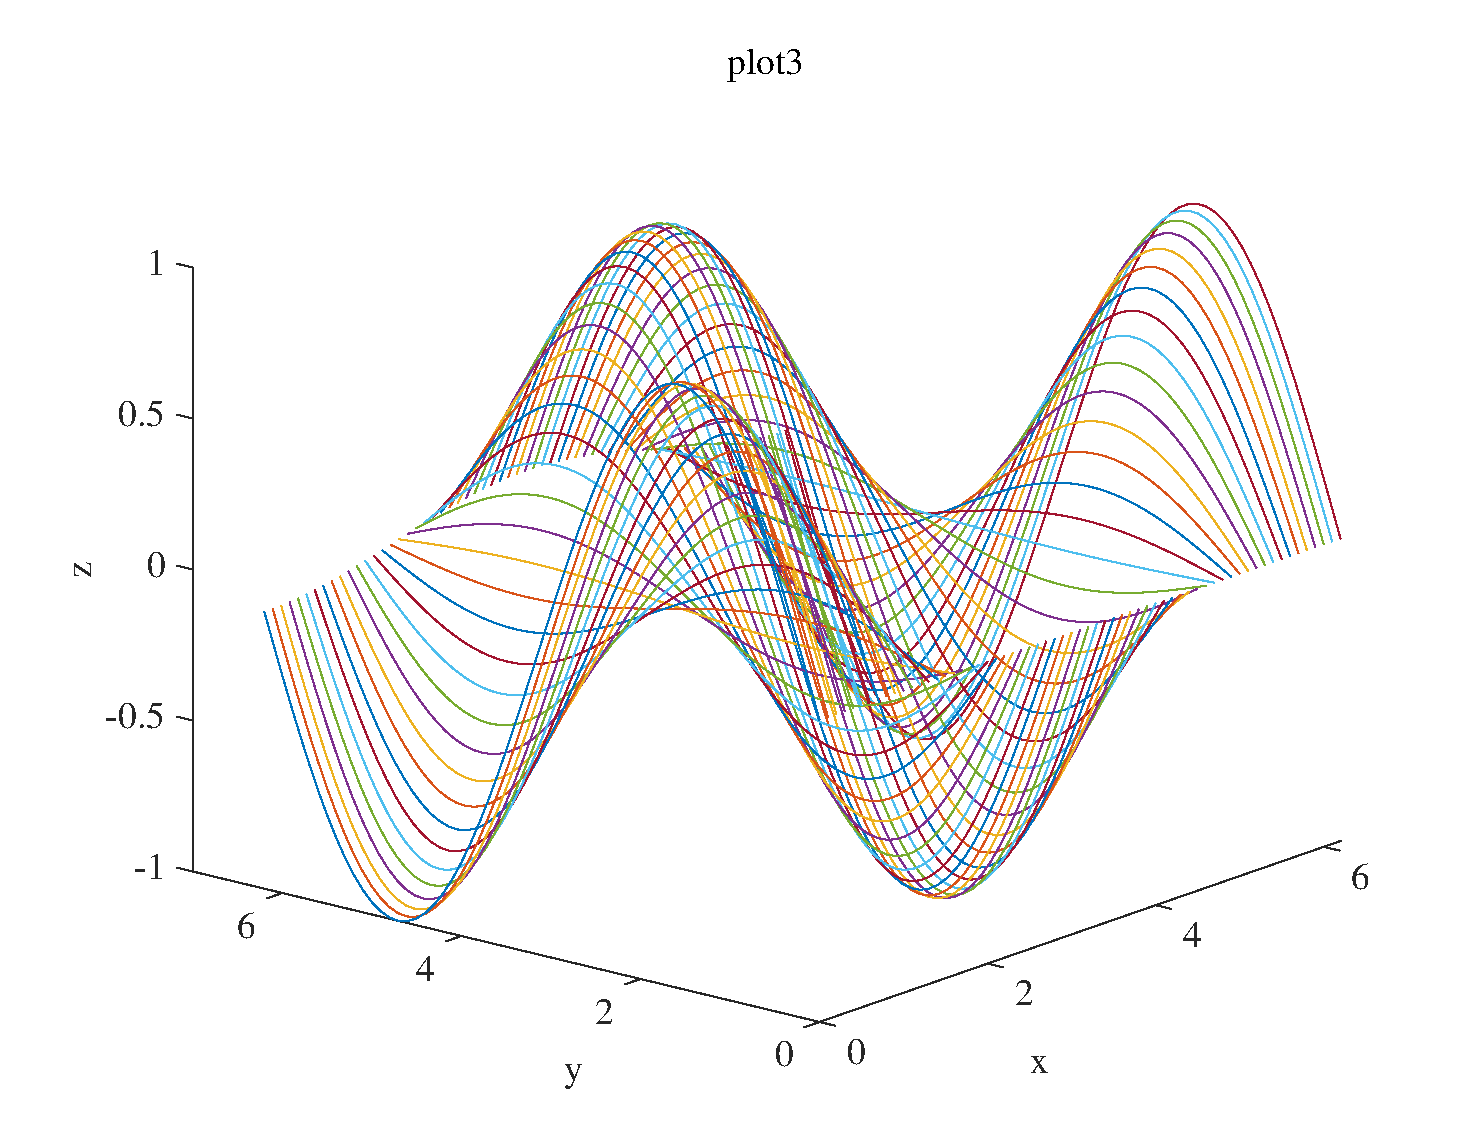
\includegraphics[width=0.6\linewidth]{pic/plot3.pdf}
	\vspace*{-2em}
	\caption{\lstinline|plot3|三维图}
\end{figure}

\subsection{其他三维图形}
特殊的三维图形与特殊二维图形的使用类似,具体使用说明见\ref{条形类} $-$ \ref{矢量类} ,常见的特殊三维图形见下表\ref{特殊三维函数}.
\begin{table}[!htb]
	\centering
	\setlength{\tabcolsep}{10mm}{
		\begin{tabular}{cl}
			\toprule
			类型 & 函数\\
			\midrule
			\multirow{2}*{三维条形图} & \lstinline|bar3(y), bar3h(y)| \\
			& \lstinline|bar3(x, y), bar3h(x, y)|\\
			三维饼图 & \lstinline|pie3(x, explode)|\\
			三维实心图 & \lstinline|fill3(x, y ,z, c)| \\
			三维散点图 & \lstinline|stem3(z), steam3(x, y, z)|\\
			三维箭头图 & \lstinline|quiver3(x, y, z, u, v, w)|\\
			瀑布图 & \lstinline|waterfall(x, y, z)|\\
			二维等高线图 & \lstinline|contour(x, y, 等级数, 选项)|\\
			三维等高线图 & \lstinline|contour3(x, y, z, 等级数, 选项)|\\
			\bottomrule
		\end{tabular}
	}
\caption{常见的特殊三维图函数}
\label{特殊三维函数}
\end{table}
例如:
\begin{lstlisting}
subplot(2, 2, 1); bar3(magic(4)); title('bar3');
subplot(2, 2, 2); pie3([2347, 1827, 2043, 3025]); title('pie 3');
a = rand(3, 5); b = rand(3, 5); c = rand(3, 5);
subplot(2, 2, 3); fill3(a, b, c, 'y'); title('fill3');
y = 2*sin(0:pi/10:2*pi);
subplot(2, 2, 4); stem3(y); title('stem3');
\end{lstlisting}
\begin{figure}[!htb]
	\centering
	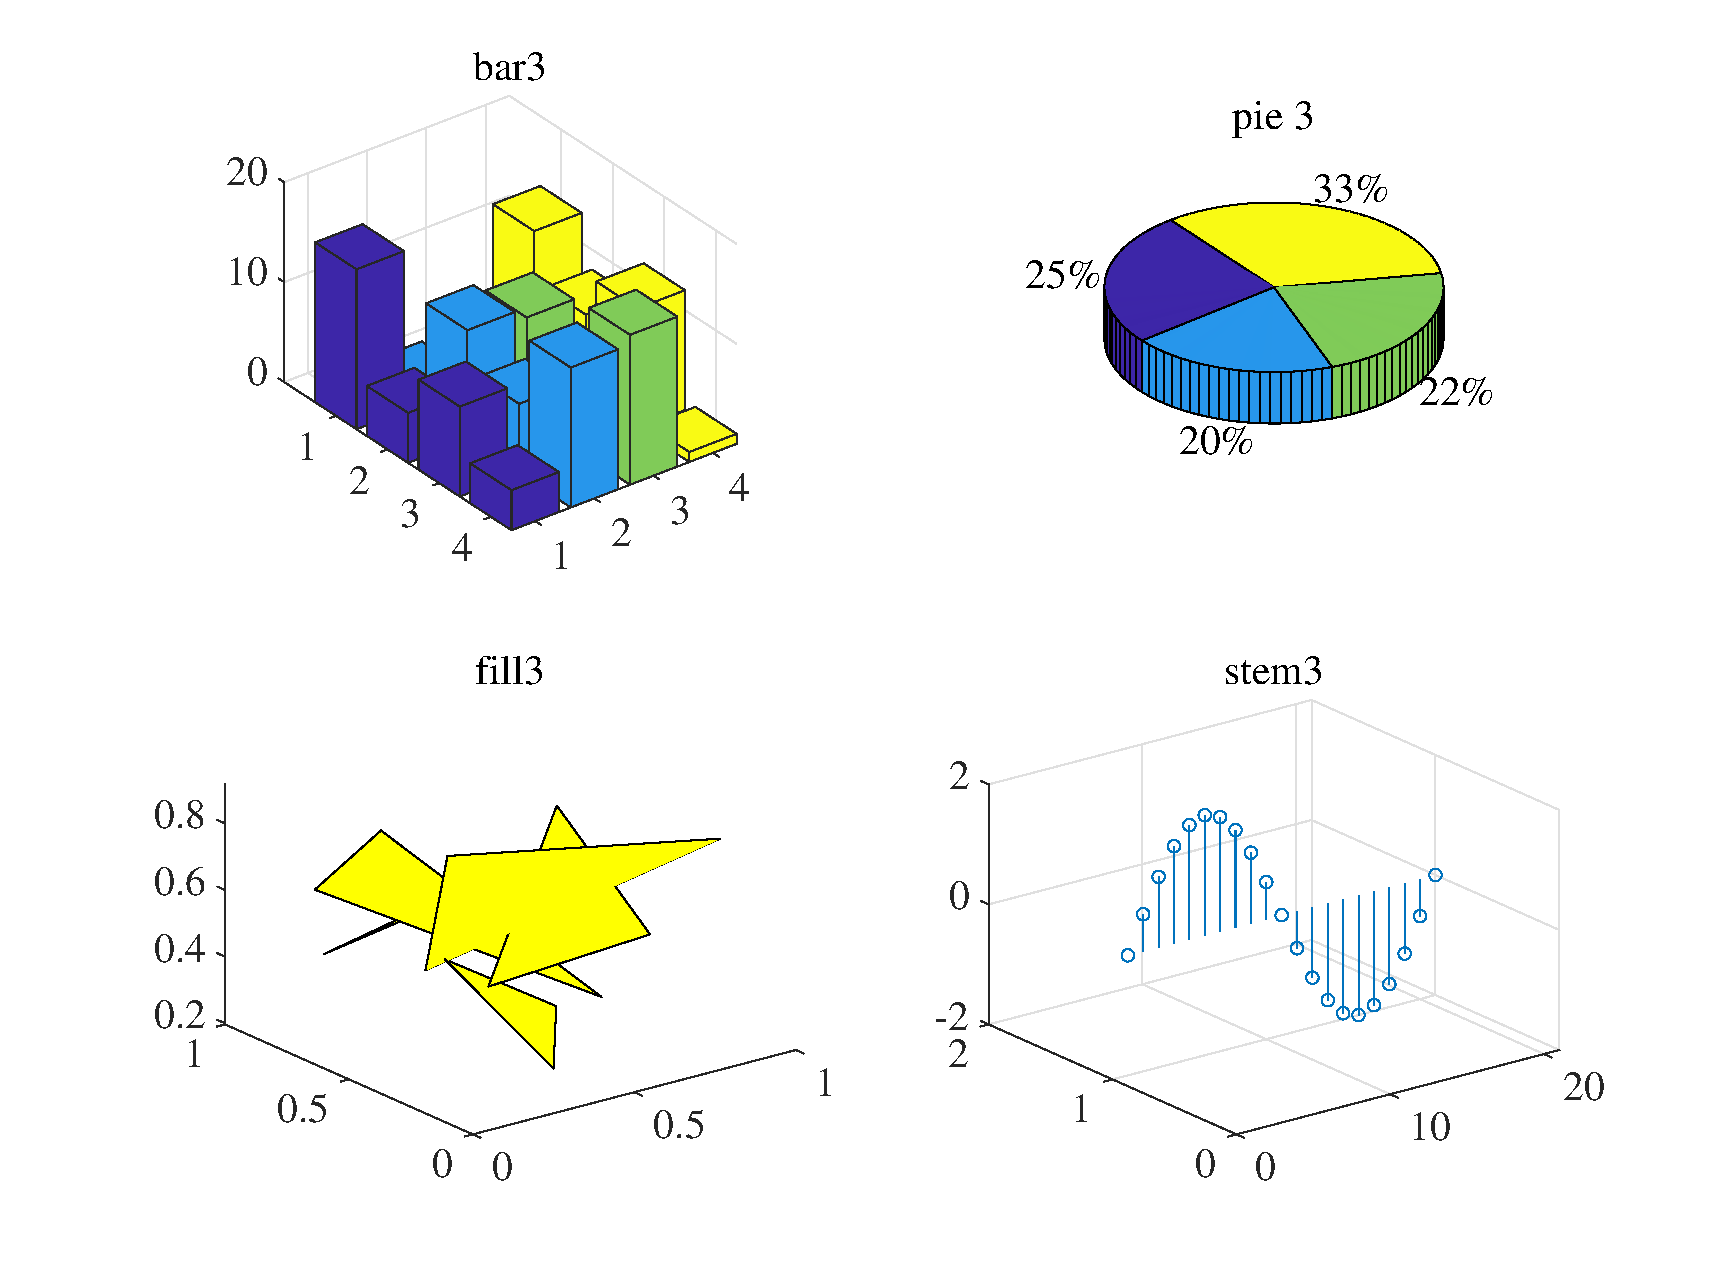
\includegraphics[width=0.9\linewidth]{pic/特殊三维图.pdf}
	\vspace*{-2em}
	\caption{特殊三维图}
\end{figure}

\section{隐函数绘图}
\subsection{隐函数二维绘图}

\noindent 隐函数用\lstinline|ezplot|进行绘图,它有各种变形如下
\begin{itemize}
	\item 隐函数$f(x)=0$
	\vspace*{-1em}
	\begin{itemize}
		\item \lstinline|ezplot(f)| 
		\begin{itemize}
			\item 在默认区间$-2 \pi < x <2\pi$ 绘制$y = f(x)$的图形
			\item $f$可以是函数文件名或函数表达式组成的字符串,也可以是匿名函数表达式或函数名
		\end{itemize}
		\item \lstinline|ezplot(f, [a,b])|
		\begin{itemize}
			\item 在区间$a < x <b\pi$ 绘制$y = f(x)$的图形
		\end{itemize}
	\end{itemize}
	\item 隐函数$f(x,y) = 0$
	\begin{itemize}
		\item \lstinline|ezplot(f)|
		\begin{itemize}
			\item 在默认区间$-2\pi < x < 2\pi, -2 \pi < y < 2 \pi$ 绘制$f(x,y)= 0$的图形
		\end{itemize}
		\item \lstinline|ezplot(f, [a, b])|
		\begin{itemize}
			\item 在区间$a< x < b, a < y < b$绘制$f(x,y) = 0$的图形
		\end{itemize}
		\item \lstinline|explot(f, [xmin,xmax, ymin, ymax])| 
		\begin{itemize}
			\item 在区间$x\min < x < x\max$和$y\min < y < y\max$绘制$f(x,y) = 0$的图形
		\end{itemize}
	\end{itemize}
	\item 参数方程$x=x(t), y = y(t)$
	\begin{itemize}
		\item \lstinline|ezplot(x, y)|
		\begin{itemize}
			\item 在默认区间$-2 \pi < t <2\pi$ 绘制$x = x(t), y = y(t)$的图形
		\end{itemize}
		\item \lstinline|ezplot(x, y, [xmin ,ymin])|
		\begin{itemize}
			\item 在区间$t\min < t < t\max$ 绘制$x = x(t), y = y(t)$的图形
		\end{itemize}
	\end{itemize}
\end{itemize}
例子
\begin{lstlisting}
subplot(2,2,1);		ezplot('x^2+y^2-9'); axis equal;
subplot(2,2,2);		ezplot(@(x, y) x^3+y^3-5.*x.*y + 1/5);
subplot(2,2,3);		ezplot('cos(tan(pi*x))', [0, 1]);
subplot(2,2,4);		ezplot('8*cos(t)', '4*sqrt(2)*sin(t)', [0, 2*pi]);
\end{lstlisting}

\begin{figure}[!htb]
	\centering
	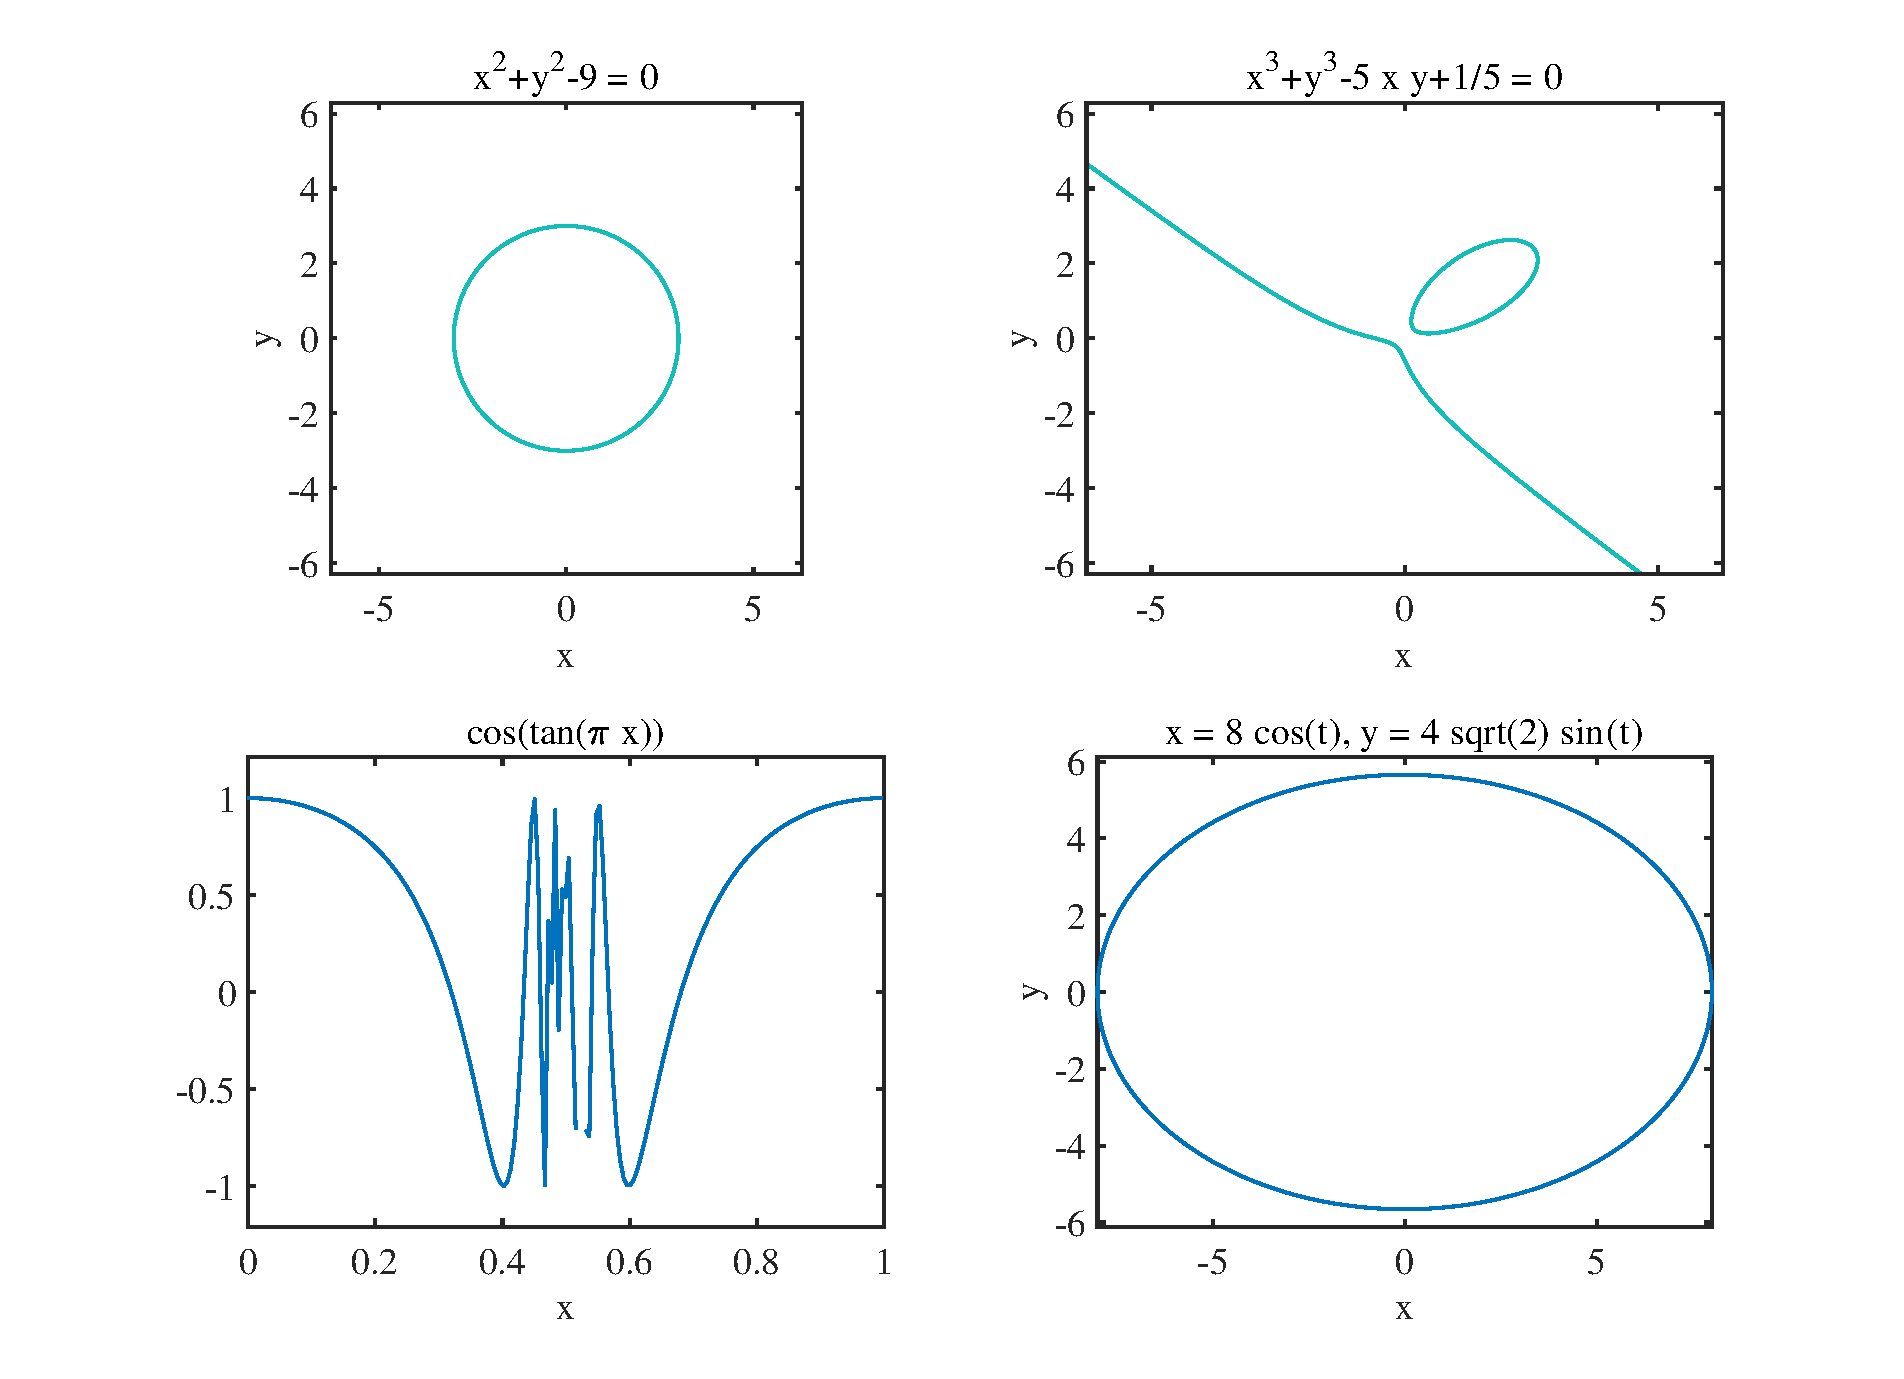
\includegraphics[width=0.8\linewidth]{pic/二维隐函数.pdf}
	\vspace*{-2em}
	\caption{二维隐函数}
\end{figure}

\subsection{三维隐函数绘图}
 隐函数三维绘图的函数有\lstinline|ezcontour, ezcontourf, ezmesh, ezmeshc, ezplot3, ezpolar, ezsurf, ezsurfc|,它们的调用格式基本相同,需要时直接查阅帮助信息。下面对\lstinline|ezsurf|进行简介
\begin{itemize}
	\item \lstinline|ezsurf(f)|  \quad 绘制曲线$z = f(x,y)$,$f$的表达与\lstinline|ezplot|函数相同,默认区间$-2\pi < x < 2\pi, -2\pi < y < 2\pi$
	\item \lstinline|ezsurf(f, [xmin,xmax, ymin,ymax]), ezsurf(f, [min,max])|\quad 在指定的区间上绘制曲线$z = f(x,y)$
	\item \lstinline|ezsurf(x, y, z)| \quad 在默认区域$-2\pi < s< 2\pi, -2\pi < s< 2\pi$上绘制参数方程$x =x (s,t), y = y(s, t), z = z(s,t)$所确定的曲面
	\item \lstinline|ezsurf(x, y, z, [smin,smax, tmin,tmax]), ezsurf(x, y, z, [min, max])| \quad 在指定的区间上绘制参数方程曲面
\end{itemize}

\examples 绘制下列曲面
\begin{align*}
	\begin{cases}
		x = \e^{-s} \cos t\\
		y = \e ^{-s} \sin t\\
		z = t
	\end{cases}
, \quad 0 \le s \le 8,0\le t \le 5\pi
\end{align*}
\begin{lstlisting}
>> ezsurf('exp(-s).*cos(t)', 'exp(-s).*sin(t)', 't', [0,8, 0,5*pi])
\end{lstlisting}
\begin{figure}[!htb]
	\centering
	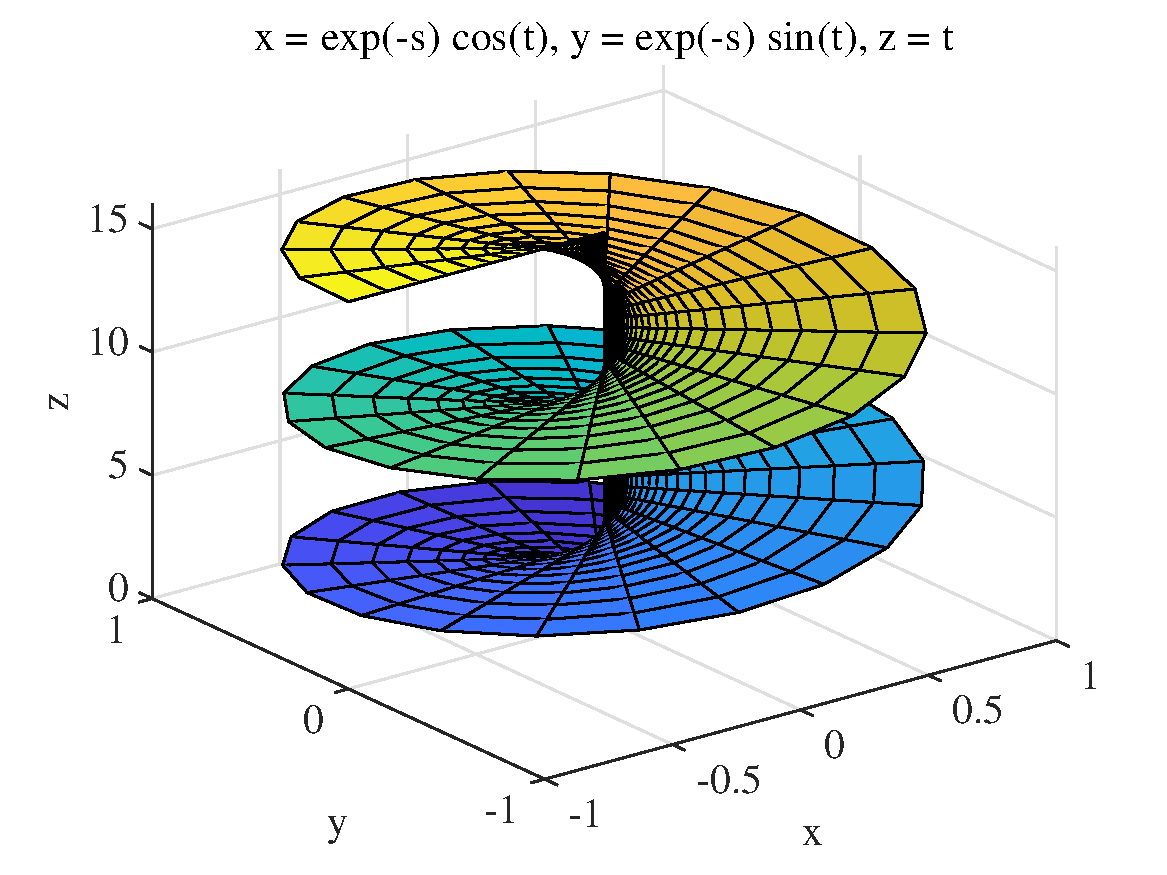
\includegraphics[width=0.8\linewidth]{pic/三维曲面.pdf}
	\caption{三维参数曲面图}
\end{figure}